\documentclass[a4paper,11pt]{article}
\usepackage[francais]{babel}
\usepackage[utf8]{inputenc}
\usepackage[T1]{fontenc}

\usepackage{graphicx}
\usepackage{amsmath,amsfonts,amssymb}
\usepackage{cases}
\usepackage{fullpage}
\usepackage{enumitem}
\usepackage{float}
\usepackage{hyperref}
\renewcommand{\baselinestretch}{1.2}

\begin{document}
\author{Adimy Y.  Simon M.  Vassal H.}
%Proposition de titre?
\title{\Huge\textbf{ Evolution de la population \\ \vspace{0.5cm} d'\textit{Homo Neanderthalensis}} \vspace{0.5cm}}
\date{Juin 2016}

\makeatletter
  \begin{titlepage}
  \centering
  	\vfill
      
\includegraphics[width=0.25\textwidth]{logo_insa.png}\\
  	\vspace{0.5cm}
      {\large \textsc{INSA de Lyon}}\\
      3ème année Bio-Informatique et Modélisation\\
    \vfill
      \textbf{\Huge\@title}\\
    \vspace{0.3cm}
      \textbf{\Large Equations de réaction-diffusion}\\
    \vspace{0.3cm}
       {\large \@author} \\
    \vspace{0.3cm}
        {\large\textbf{\@date}}\\
    \vfill
    	\centering
        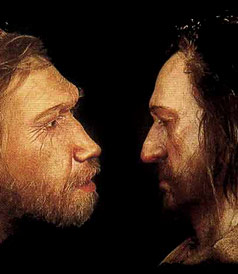
\includegraphics[scale=1]{neanderthal-sapiens.jpg}
  \end{titlepage}
\makeatother
\newpage
\tableofcontents
\newpage

\setcounter{page}{1}

\section{Contexte biologique}
\begin{center}
	\textbf{\textit{Pourquoi l'homme de Néandertal a-t-il disparu ? }}
\end{center}

Il s'agit là de la disparition la plus fascinante de l’histoire de l’humanité. Pourquoi, après avoir vécu 120 000 ans, l'homme de Néandertal a-t-il mystérieusement disparu, au moment-même de sa cohabitation avec les Hommes modernes en Europe?  Comment s'est passé cette extinction et pourquoi Néandertal n'a-t-il pas continué de vivre en cohabitation avec Sapiens ? 
	 
Nous nous sommes donc intéressées à l'évolution de la population de l'Homme de Néandertal, durant le stade isotopique 3 (période interglacière d'environ -60 000 à -30 000). Cette étude porte en fait sur la période de la transition entre le paléolithique moyen (de -300 000 à -30 000 ans avant le présent) et  le paléolithique supérieur (entre -45 000 et -10 000 ans avant le présent). A cette période l'Homme de Néandertal avait colonisé une grande partie de l'Europe ce qui a pu être constaté par la découverte de nombreux sites archéologiques présentant des traces de l'Homme de Néandertal. La carte ci-dessous (Figure \ref{C1}) permet de situer ceux présentant des traces datant de -50000 à -40000. \\
 
\begin{figure}[H]
	\centering
    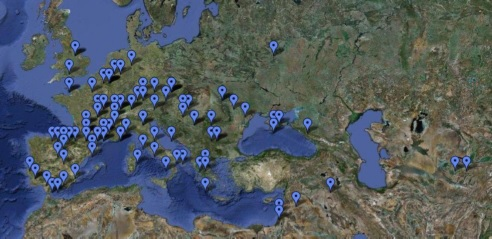
\includegraphics[width=10cm]{SiteArche.jpg}
    \caption{Répartition des sites archéologiques de -50000 à -40000 ans}
    \label{C1}
\end{figure}
La période étudiée ici correspond à l'arrivée de \textit{Homo Sapiens} en Europe et à la disparition progressive de \textit{Homo Neanderthalensis}. Nous avons ainsi tenté de comprendre quelles pouvaient êtres les causes de cette extinction. Parmi les hypothèses possibles figurent le climat et la compétition avec l'Homme Moderne. Ce dernier aurait finalement survécu face à l'Homme de Néandertal grâce à un régime alimentaire moins restreint, une agressivité plus développée et des innovations techniques plus performantes, ce qui lui aurait permis de faire face au stress climatique.\\
Nous avons d'abord souhaité étudier plusieurs modèles permettant d'étudier la population de  l'Homme de Néandertal sans compétition avec l'Homme Moderne (modèle de la croissance Logistique et modèle avec effet Allee). Nous avons ensuite tenté de développer un modèle de compétition à deux populations (Lotka-Volterra) afin de modéliser l'interaction entre les deux populations d'Homme à cette époque. D'autres modèles, plus compliqués à étudier, pourraient être appliqués prenant en compte l'âge des populations, ou le climat par exemple.


\section{Présentation des modèles étudiés}
\subsection{Cadre général}
Le but de notre projet est d'étudier l'évolution de la population de Néandertal en la modélisant par une équation de réction-diffusion du type : \\
\begin{equation}
\frac{\partial u(t,x)}{\partial t}=f(u(t,x))+d\Delta u(t,x), \quad t \in \mathbb{R}, x \in \mathbb{R} \\
\end{equation}
La fonction inconnue u représente la densité de population dans un espace donné. Il s'agit donc d'un nombre d'habitants par kilomètre carré. En théorie, $u\in [0;+\infty]$. Toutefois, en pratique et dans le cas considéré (population d'Homme de Néandertal et d'\textit{Homo Sapiens}),$u\in [0;1]$. Nous limiterons donc notre étude à cet intervalle.\\
\newline
Il est important dans un premier temps de comprendre l'évolution de la densité de population par rapport au temps. En supposant que le temps est continu on obtient des équations différentielles ordinaires que nous pouvons étudier. $f(u(t,x))$ correspond à la partie réaction qui modélise la croissance de la population. On proposera différentes fonction $f$ en fonction des différents modèles de croissance de population utilisés. Cette fonction dépend de la croissance de la population, mais peut aussi faire intervenir des facteurs limitants. D'autre part, on peut aussi modéliser les interactions entre plusieurs populations en étudiant des systèmes
d'équations differentielles.\\
\newline
On ne s'intéresse pas à l'apparition de la population sur le territoire. Dans tout notre projet, nous avons considéré une fonction $f: \mathbb{R} \times \mathbb{R}^+ \to \mathbb{R}$  de classe $C^1$. \\

On doit ensuite incorporer les mouvements dans l'espace de la population. Pour cela, on souhaite modéliser la marche aléatoire des individus. Chaque marche aléatoire suit une loi particulière mais de manière générale l'agglomérat de population se déplace selon un processus macroscopique que l'on nomme processus de diffusion.
L'ajout d'un terme de diffusion $d\Delta u(t,x)$ permet ainsi de modéliser le mouvement aléatoire des individus dans l'espace.\\
\newline
 En combinant ces deux processus de reaction f et  de  diffusion, on obtient une équation de réaction-diffusion.
On considère donc le problème de Cauchy suivant : 
\begin{equation}\label{PbCauchy}
\left\{
\begin{array}{r c l}
 \frac{\partial u(t,x)}{\partial t}&=&f(u(t,x))+d\Delta u(t,x)\\
u(0,.) &=& u_0\\
\end{array}
\right.
\end{equation}
L'objectif principal est de déterminer les situations où l'espèce \textit{Homo Neanderthalensis} s'éteint. Mathématiquement, cela nécessite de caractériser l'état de l'équilibre 0. On pourra traiter deux types de stabilité dans notre travail.
On dit que l'état d'équilibre 0 est uniformément asymptotiquement stable si pour une condition initiale $u_0$ assez proche de 0, la solution u de \ref{PbCauchy} converge uniformément vers 0 quand t tend vers l'infini. On dit aussi que l'état 0 est inconditionellement stable dans le cas où cette convergence vers 0 est vérifiée quelque soit la condition intiale $u_0$. Pour répondre à notre problème, le premier type de stabilité mentionné ici est plus restrictif que le second car il nécessite que la population ne soit pas trop grosse pour qu'elle puisse s'éteindre.   



\subsection{Croissance Logistique}
Dans les années 1840, Pierre François Verhulst proposa un modèle permettant de modéliser la croissance d'une population. L'équation logistique est une équation différentielle ordinaire qui est l'un des modèles les plus simples de dynamique des populations. On suppose que les naissances et les morts sont proportionnelles à la taille de la population, et qu'il n'y a pas de migration. Ce modèle permet d'intégrer une notion de saturation de l'environnement, qui témoigne en fait de l'existence d'un effectif maximum pour une population (dépendant essentiellement des conditions de subsistance du milieu). 

Nous l'avons appliqué ici en ajoutant un terme de diffusion.

$$\frac{\partial u(t,x)}{\partial t}=f(u(t,x))+d\Delta u(t,x)$$
$$\text{Avec : }f(u(t,x))=\alpha u (1 - \dfrac{u}{K}) $$

\noindent où u(t,x) représente la densité de population au temps t et à la position x.\\

\noindent $K$ : Capacité de transport liée à des facteurs locaux environnementaux ($K$>0) \\
$\alpha$ : Taux de croissance maximum intrinsèque de la population. ($\alpha$>0)\\
$d$ : Constante de diffusion qui précise le taux de dispersion spatiale moyen des individus entre leur naissance et leur reproduction.($d$>0)

\subsection{Effet Allee}
Le modèle à croissance logistique n'est pas forcément adapté pour une population humaine. En effet, lorsque les densités sont faibles, le risque d'extinction est plus grand. Ceci s'explique par l'apparition d'un effet de groupe qui peut influencer la fertilité ou la survie. Cette corrélation entre la densité de population et son taux de croissance peut être caractérisée par l'effet Allee.\\
Pour des populations telles que les populations humaines, où la structure sociale a une grande influence, l'effet Allee peut être très important. On considère ici un effet Allee fort.

$$\frac{\partial u(t,x)}{\partial t}=f(u(t,x))+d\Delta u(t,x)$$
$$\text{Avec : }f(u(t,x))=ku(1-u)(u-A)$$

\noindent $u$: Densité de population de l'Homme de Néandertal au temps t et à la position x,  $0\le u \le 1$\\
$k$ : Taux de croissance normalisé constant \\
$A$ : Densité critique en dessous de laquelle le taux de croissance de la population devient négatif, $0\le A \le 1$
\vspace{0.5cm}\\
Dans le cas où le taux de croissance maximum per capita vaut 1, c-à-d $max_{0\le u \le 1} f(u)/u=1$, on peut exprimer $k$ en fonction de $A$ : 
\begin{equation}
k=\frac{4}{(1-A)^2}
\label{Eqk}
\end{equation}

\subsection{Système de Lotka-Volterra}
On sait que \textit{Homo sapiens} et \textit{Homo Neanderthalensis} ont connu une période de cohabitation, située entre l’apparition du premier véritable Homme Moderne (il y a 45.000 ans) et l’extinction de l'Homme de Néandertal (il y a 40.000 ans). Nous nous sommes intéressées aux interactions entre ces deux populations à l'aide du système de Lotka-Volterra. Dans ce modèle, on considère que les populations sont en compétition.\\
$$\begin{cases} \frac{\partial u(t,x)}{\partial t} = f(u,v) + d_1\Delta u\\ \frac{\partial v(t,x)}{\partial t} = g(u,v) + d_2 \Delta v \\ 
\end{cases}$$
$$\text{Avec : } f(u,v) = \alpha_1 u\left(1-\frac{u}{K_1}-\gamma_1\frac{v}{K_1}\right) \text{ et } g(u,v) = \alpha_2 v\left(1-\frac{v}{K_2}-\gamma_2\frac{u}{K_2}\right)$$
$u$ : Densité de population des Hommes Modernes \\
$v$ : Densité de population des Hommes de Néandertal.\\
$K_1$ et $K_2$ : Capacités d'accueil du milieu\\
$\gamma_1$ et $\gamma_2$ : Coefficients de compétition\\
$\alpha_1$ et $\alpha_2$ : Taux de croissance\\

\noindent Tous les paramètres sont positifs.

\section{Analyse mathématique}
\subsection{Croissance Logistique}
\subsubsection{Analyse de la partie réaction}

On étudie d'abord les points d'équilibre et leur stabilité pour l'équation sans diffusion : $$\frac{du}{dt}=\alpha u (1- \dfrac{u}{K})$$
avec $\alpha>0$ et $K>0$.
\newline

\noindent\underline{Equilibres :} Les équilibres sont les fonctions u qui vérifient $\frac{du}{dt}=0$. On a donc :
\[
\left\{
\begin{array}{r c l}
u_0 &=& 0\\
u_K &=& K\\
\end{array}
\right.
\]
\underline{Stabilité :} On étudie le signe de $f'(u)$ 
$$f^\prime(u)= \alpha - 2 \alpha \dfrac{u}{K} $$

\begin{itemize}
    	\item[*] $f^\prime(0)=\alpha >0 \Rightarrow $ équilibre instable
        \item[*] $f^\prime(K)= -\alpha <0 \Rightarrow $ équilibre stable
	\end{itemize}


\subsubsection{Analyse de la réaction-diffusion}
\setcounter{equation}{0}
L'idee est de representer la solution de notre equation de
reaction-diusion sous forme d'un front qui se deplace dans l'espace a une vitesse constante.
Soit u la solution de notre équation de reaction-diffusion dans $\mathbb{R}$.

\noindent On pose $z=x-ct$, $U:z\rightarrow U(z)$.\\
On ecrit alors notre solution sous la forme
\begin{equation}
u(t,x)=U(x-ct)=U(z)
\label{Eq1}
\end{equation}
U est la forme de l'onde et c sa vitesse.\\

On peut montrer (Voir Annexe 1) que ~\eqref{Eq1} est équivalent à :
\begin{equation*}
dU"(z)+c U'(z)+\alpha U(z)(1-\dfrac{U(Z)}{K})=0\\
\end{equation*} 

On a donc (U, c) solution du problème suivant :
\begin{equation} 
\left\{
\begin{array}{lcl}
dU"(z)+c U'(z)+\alpha U(z)(1-\dfrac{U(Z)}{K})=0 \\
U( - \infty )= K ,\quad U( + \infty )=0
\end{array}
\right.
\label{PbKPP }
\end{equation}
On dira que c est la vitesse de propagation. Ces solutions décrivent donc l'invasion de l'état K
sur 0 si $c > 0$ ou de l'état 0 sur K si $c< 0$, selon un profil constant qui se déplace à la vitesse
$|c|$.\\
\newline

\begin{figure}[H]
	\centering
	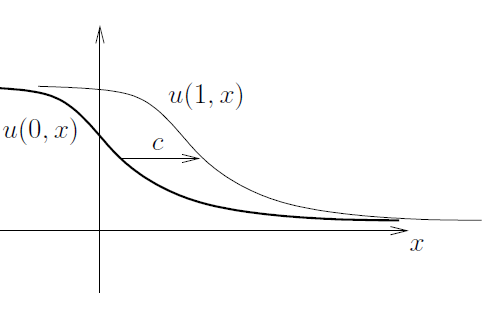
\includegraphics[width=0.40\linewidth]{SimulationKPP/FrontOnde}\hfill
	\caption{Profil U se déplacant à la vitesse c}
\end{figure}



On pose $V=U' \Rightarrow V'=U"$:
\[
\left\{
\begin{array}{r c l}
U' &=& V\\
V' &=& \dfrac{1}{d} \times (-\alpha U(Z) + \dfrac{\alpha}{K} U^2(Z)- c V(Z))
\end{array}
\right.
\]
On a donc : $W'=F(W)$ avec $W=\begin{pmatrix} U \\ V \end{pmatrix}$\\ et $F(W)=\begin{pmatrix} f_1(U,V) \\ f_2(U,V) \end{pmatrix}=\begin{pmatrix} V \\ \dfrac{1}{d} \times (-\alpha U(Z) + \dfrac{\alpha}{K} U^2(Z)- c V(Z)) \end{pmatrix}$
\newline
\newline
\underline{Recherche des équilibres}


\[
F(W)=0 \Rightarrow
\left\{
\begin{array}{r c l}
V &=& 0\\
U &=& 0 \quad \text{  ou } \quad U = K
\end{array}
\right.
\]
Ainsi on a deux points d'équilibre $(0,0)$ et $(K,0)$
\newline
\newline
\underline{Stabilité}\\
Matrice jacobienne : $$\mathcal{J}_{F_{(U,V)}}=\begin{pmatrix} 0 & 1 \\ -\dfrac{\alpha}{d}+ \dfrac{2 \alpha U }{d K} & -c\end{pmatrix}$$
\newline
\begin{itemize}[label=$\bullet$]
	\item$\mathcal{J}_{F_{(K,0)}}=\begin{pmatrix} 0 & 1 \\ \frac{\alpha}{d} & -c \end{pmatrix}$\\
    \begin{itemize}
		\item[*] $det (\mathcal{J}_{F_{(K,0)}}) = - \frac{\alpha}{d} <0$. $(0,0)$ est donc un point selle.
	\end{itemize}
    \item $\mathcal{J}_{F_{(0,0)}}=\begin{pmatrix} 0 & 1 \\ - \frac{\alpha}{d} & -c \end{pmatrix}$\\
    \begin{itemize}
		\item[*] $tr (\mathcal{J}_{F_{(0,0)}})= -c <0$. 
        \item[*] $det (\mathcal{J}_{F_{(0,0)}}) = \frac{\alpha}{d}>0 $\\
    \end{itemize}
\noindent Ici on peut juste dire que le point est stable.
Pour connaître la nature du point, il faut étudier le déterminant : $\Delta = tr^2 -4 det= c^2-4 \frac{\alpha}{d}$\\
            c est une vitesse, elle est donc positive. Ainsi on a :
      	\begin{itemize}[label=$\rightarrow$]
			\item si $c>2\sqrt{\frac{\alpha}{d}} \Rightarrow \Delta >0$ : Noeud Localement Asymptotiquement Stable
            \item si $c=2\sqrt{\frac{\alpha}{d}} \Rightarrow \Delta =0$ : Etoile ou Noeud Dégénéré Asymptotiquement Stable
            \item si $0<c<2\sqrt{\frac{\alpha}{d}} \Rightarrow \Delta <0$ : Foyer Asymptotiquement Stable. Cependant U étant une population, elle ne peut être négative. Or avec un Foyer assymptotiquement stable autour de l'équilibre (0,0) U deviendrait négatif. On ne considère donc pas ce cas.
		\end{itemize}
\end{itemize}

\underline{Etude des fronts d'ondes}\\
$$f(u)= \alpha u (1 - \dfrac{u}{K})$$
$$f^\prime(u)= \alpha - 2 \frac{\alpha u}{K}$$


Dans un premier temps on a $$ f(u) - f'(0)u = \alpha u (1 - \dfrac{u}{K}) - \alpha u = u\alpha (- \dfrac{u}{K}) < 0$$

On donc a  $f(u) < f'(0)u$, $f(0) = f(K) = 0$ et f est positive sur [0,K]. Cette fonction est donc de classe KPP.

\begin{figure}[H]
	\centering
	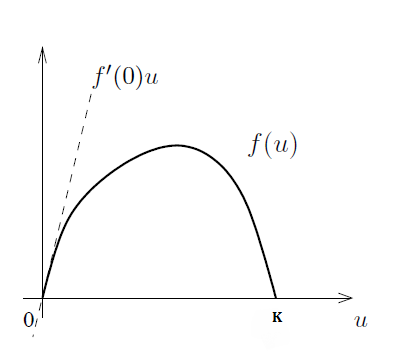
\includegraphics[width=0.40\linewidth]{SimulationKPP/fu}\hfill
	\caption{Fonction de type KPP}
\end{figure}


f possède deux équilibres $0$ et $K$ tels que $0 < K$ :\\
	\begin{itemize}
    	\item[*] $f^\prime(0)= \alpha >0 \Rightarrow $ 0 est instable
        \item[*] $f^\prime(K)= -\alpha <0 \Rightarrow $ K est stable\\
	\end{itemize}
    
    
    Le plus petit équilibre $0$ est instable et le plus grand $K$ est stable donc l'équation de réaction-diffusion est \textbf{monostable}. \\

Dans le cas KPP et monostable on a l'existence d'un continuum de vitesses c tel que le probleme (\ref{PbKPP }) a une solution, et donc une infinite de solutions (U,c). Plus precisesement, pour le cas KPP et monostable, il existe un vitesse minimale c$_0 >0$ unique telle que quelque soit $c  \geqslant c_0$ l'equation (\ref{PbKPP }) a une solution $U_c$ unique a translation près.

    Il existe donc une vitesse minimale $c_0$ telle que pour toute vitesse supérieure, on a existence d'un front d'onde U(z) monotone, solution de l'EDO avec les conditions aux bords $\lim_{z \to +\infty} U(z)=0$ et $\lim_{z \to -\infty} U(z)=K$. \\
    
    De plus comme $ f^\prime(u)< f^\prime(0)$ pour un voisinnage de $0$ alors : \\
    $c_0=2 \sqrt{f^\prime(0)}= 2 \sqrt{\alpha - 2 \frac{\alpha}{K} \times 0} = 2 \sqrt{\alpha}$\\
    On peut donc déterminer la vitesse de cette propagation. \\
    
    
        D'autre part, comme l'équation est monostable avec aucun autre équilibre entre $0$ et $K$, si on prend comme condition initiale l'équilibre instable $0$ avec une perturbation à support borné, alors la solution tend vers deux fronts de vitesse minimale $c_0$. \\
		On appelle cet effet l'effet "hair trigger effect". Ainsi, dans le cas KPP et monostable il suffit que
		la condition initiale soit non équivalente à 0 , c'est à dire décolle légèrement de 0, pour que la solution
		converge vers K à la vitesse c$_0$. 
		
		
		
\subsection{Effet Allee}
\subsubsection{Analyse de la partie réaction}
On étudie d'abord les points d'équilibre et leur stabilité pour l'équation sans diffusion : $$\frac{du}{dt}=ku(1-u)(u-A)$$
\underline{Equilibres :} Les équilibres sont les fonctions u qui vérifient $\frac{du}{dt}=0$. On a donc :
\[
\left\{
\begin{array}{r c l}
u_0 &=& 0\\
u_1 &=& 1\\
u_A &=& A\\
\end{array}
\right.
\]
\underline{Stabilité :} On étudie le signe de $f'(u)$ 
$$f^\prime(u)= -3ku^2 + 2k(1+A)u-kA$$

\begin{itemize}
    	\item[*] $f^\prime(0)=-kA <0 \Rightarrow $ stable
        \item[*] $f^\prime(1)=kA(1-A) <0 \Rightarrow $ stable
        \item[*] $f^\prime(A)=k(A-1) >0 \Rightarrow $ instable
	\end{itemize}

\subsubsection{Analyse de la réaction-diffusion}
\noindent On pose $z=x-ct$, $U:z\rightarrow U(z)$.\\
On a alors : 
\begin{equation}
u(t,x)=U(x-ct)=U(z)
\tag{1}
\label{Eq1}
\end{equation}
U est la forme de l'onde et c sa vitesse.\\
On peut montrer (Voir Annexe 1) que ~\eqref{Eq1} est équivalent à :
\begin{equation}
dU"(z)+cU'(z)+kU(z)(1-U(z))(U(z)-A)
\tag{2}
\end{equation} 
On pose $V=U' \Rightarrow V'=U"$:
\[
\left\{
\begin{array}{r c l}
U' &=& V\\
V' &=& -\frac{c}{d}V-kU(1-U)(1-A)
\end{array}
\right.
\]
On a donc : $W'=F(W)$ avec $W=\begin{pmatrix} U \\ V \end{pmatrix}$ et $F(W)=\begin{pmatrix} f_1(U,V) \\ f_2(U,V) \end{pmatrix}=\begin{pmatrix} V \\ -\frac{c}{d}V-kU(1-U)(1-A) \end{pmatrix}$
\newline
\newline
\underline{Recherche des équilibres}\\
$F(W)=0 \Rightarrow V=0 \Rightarrow U=0 \text{ ou } U=1 \text{ ou } U=A$.\\
Cependant, u et A représentent des densités donc ils sont inférieurs à 1. Il faut donc distinguer deux cas :
\begin{itemize}
	\item $A<1$, le système admet trois équilibres $(0,0)$, $(A,0)$ et $(1,0)$.
    \item $A=1$, le système admet deux équilibres $(0,0)$ et $(1,0)$.
\end{itemize}
\vspace{0.5cm}
\underline{Stabilité}\\
Matrice jacobienne : $$\mathcal{J}_{F_{(U,V)}}=\begin{pmatrix} 0 & 1 \\ 3kU^2-2k(1+A)+kA & -\frac{c}{d}\end{pmatrix}$$
\newline
\begin{itemize}[label=$\bullet$]
	\item$\mathcal{J}_{F_{(0,0)}}=\begin{pmatrix} 0 & 1 \\ kA & -\frac{c}{d} \end{pmatrix}$\\
    \begin{itemize}
		\item[*] $det (\mathcal{J}_{F_{(0,0)}}) = -kA <0$. $(0,0)$ est donc d'un point selle.
	\end{itemize}
    \item $\mathcal{J}_{F_{(1,0)}}=\begin{pmatrix} 0 & 1 \\ k(1-A) & -\frac{c}{d} \end{pmatrix}$\\
    \begin{itemize}
		\item[*] $tr (\mathcal{J}_{F_{(1,0)}})= -\frac{c}{d} <0$. 
        \item[*] $det (\mathcal{J}_{F_{(1,0)}}) = k(A-1)$
        \begin{itemize}[label=$\blacktriangleright$]
			\item $A<1 \Rightarrow det (\mathcal{J}_{F_{(0,0)}})<0$. $(1,0)$ est alors un point selle.
            \item $A=1 \Rightarrow det (\mathcal{J}_{F_{(0,0)}})=0$. La linéarisation prévoit des centres.
		\end{itemize}
	\end{itemize}
    \item $\mathcal{J}_{F_{(A,0)}}=\begin{pmatrix} 0 & 1 \\ kA(A-1) & -\frac{c}{d} \end{pmatrix}$\\
    \begin{itemize}
		\item[*] $tr (\mathcal{J}_{F_{(1,0)}})= -\frac{c}{d} <0$. 
        \item[*] $det (\mathcal{J}_{F_{(1,0)}}) = kA(1-A)$
        \begin{itemize}[label=$\blacktriangleright$]
            \item $A=1 \Rightarrow det (\mathcal{J}_{F_{(0,0)}})=0$. La linéarisation prévoit des centres.
            \item $A<1 \Rightarrow det (\mathcal{J}_{F_{(0,0)}})>0$. Pour connaitre la nature du point, il faut étudier le déterminant : $\Delta = tr^2 -4 det= \frac{c}{d}^2+4kA(A-1)$\\
            On pose $c_1=2d\sqrt(kA(1-A))=4d\sqrt{\frac{A}{1-A}}$ d'après \eqref{Eqk}
            \begin{itemize}[label=$\rightarrow$]
				\item $c>c_1 \Rightarrow \Delta >0$ : Noeud Localement Asymptotiquement Stable
                \item $c=c_1 \Rightarrow \Delta =0$ : Etoile ou Noeud Dégénéré Asymptotiquement Stable
                \item $c<c_1 \Rightarrow \Delta <0$ : Foyer Asymptotiquement Stable. Toutefois, ce cas n'est pas possible car U deviendrait négatif. Or U étant une population, il est forcément positif.
			\end{itemize}
		\end{itemize}
	\end{itemize}
\end{itemize}

\noindent \underline{Etude des fronts d'ondes}\\
Comme on l'a montré dans la partie sans diffusion, l'équation admet trois équilibres :

$$u_+=1 \text{ stable,} u_-=0 \text{ stable,} u_s=A \text{ instable}$$
	
    Donc l'équation ERD est \textbf{bistable}. Il existe un seul équilibre $u_s$ entre $u_+$ et $u_-$ \\
    Donc il existe une unique vitesse $c$ et une unique forme $U(z)$ monotone et solution de l'EDO avec les conditions aux bords $\lim_{z \to +\infty} U(z)=u_+$ et $\lim_{z \to -\infty} U(z)=u_-$. 
    
    De plus: 
	\begin{align*}
		\int_{0}^1 f(u)\, \mathrm{d}u &=\left[\frac{-ku^4}{4}+\frac{k(1+A)u^3}{3}-\frac{kAu^2}{2}\right]_0^1\\
		&=\frac{k}{12}(1-2A)
	\end{align*}
    	\begin{itemize}
        	\item[*] $\frac{1}{2}<A<1 \Rightarrow \int_{0}^1 f(u)\, \mathrm{d}u<0 \Rightarrow c<0$ : "0 envahit 1"
            \item[*] $A<\frac{1}{2} \Rightarrow \int_{0}^1 f(u)\, \mathrm{d}u>0 \Rightarrow c>0$ : "1 envahit 0"
            \item[*] $A=\frac{1}{2} \Rightarrow c=0$
		\end{itemize}




\subsection{Système de Lotka-Volterra}
\subsubsection{Analyse préliminaire}
On étudie d'abord les points d'équilibre et leur stabilité pour les équations suivantes, afin de faciliter l'étude des fronts d'onde et déterminer les paramètres pertinents :
$$\begin{cases}
\frac{\partial u}{\partial t} = f(u,v) = \alpha_1 u\left(1-\frac{u}{K_1}-\gamma_1\frac{v}{K_1}\right)\\
\frac{\partial v}{\partial t} = g(u,v) = \alpha_2 v\left(1 - \frac{v}{K_2} - \gamma_2\frac{u}{K_2}\right)
\end{cases}$$
\noindent \underline{Equilibres :}\\

$\begin{cases}
\frac{\partial u}{\partial t} = 0\\
\frac{\partial v}{\partial t} = 0
\end{cases} \Leftrightarrow \
\begin{cases}
f(u,v)=0\\
g(u,v)=0
\end{cases} \Leftrightarrow \
\begin{cases}
u = 0 \text{ ou } u = K_1 - \gamma_1 v\\
v = 0 \text{ ou } v = K_2 - \gamma_2 u
\end{cases}$\\

\noindent Les points d'équilibre sont : $(0,0)$, $(0,K_2)$, $(K_1,0)$, $(u^*,v^*)$ avec 
$u^* = \dfrac{K_1 - \gamma_1 K_2}{1-\gamma_1 \gamma_2}$ \\
et $v^* = \dfrac{K_2 - \gamma_2 K_1}{1-\gamma_1 \gamma_2}$.\\ 

D'un point de vue biologique, l'existence du dernier équilibre $(u^*,v^*)$ dépend des valeurs choisies pour les paramètres. Il faut avoir $\gamma_1\gamma_2 \neq 1$, et $(\gamma_1,\gamma_2) < \left(\frac{K_1}{K_2},\frac{K_2}{K_1}\right)$ 
ou $(\gamma_1,\gamma_2) > \left(\frac{K_1}{K_2},\frac{K_2}{K_1}\right)$.\\

\noindent \underline{Stabilité :}
La matrice Jacobienne s'écrit : $$\mathcal{J}_{(u,v)}=\begin{pmatrix} \alpha_1\left(1-\dfrac{2}{K_1}u-\dfrac{\gamma_1}{K_1}v\right) & -\dfrac{\alpha_1\gamma_1}{K_1}u \\ -\dfrac{\alpha_2\gamma_2}{K_2}v & \alpha_2\left(1- \dfrac{2}{K_2}v-\dfrac{\gamma_2}{K_2}u\right)\end{pmatrix}$$
\begin{itemize}[label=$\bullet$]
\item $\mathcal{J}_{(0,0)} = \begin{pmatrix} \alpha_1 & 0 \\ 0 & \alpha_2 
\end{pmatrix}$
 : l'équilibre est instable. Si $\alpha_1 \neq \alpha_2$, on peut dire que c'est un Noeud Instable.
 
 \item $\mathcal{J}_{(K_1,0)} = \begin{pmatrix} -\alpha_1 & -\alpha_1\gamma_1 \\ 0 & \alpha_2\left(1- \dfrac{\gamma_2 K_1}{K_2}\right)
\end{pmatrix} $\\
\begin{itemize}
  \item[*] Si $\gamma_2 < \frac{K_2}{K_1}$, $det(\mathcal{J}_{(K_1,0)}) < 0$ : c'est un Point Selle.
  \item[*] Sinon, l'équilibre est asymptotiquement stable.\\
  \end{itemize}
  
\item $\mathcal{J}_{(0,K_2)} = \begin{pmatrix} \alpha_1\left(1-\dfrac{\gamma_1 K_2}{K_1}\right) & 0 \\ -\alpha_2\gamma_2 & -\alpha_2 \end{pmatrix}$\\
  \begin{itemize}
  \item[*] Si $\gamma_1 < \frac{K_1}{K_2}$, $det(\mathcal{J}_{(0,K_2)}) < 0$ : c'est un Point Selle.
  \item[*] Sinon, l'équilibre est asymptotiquement stable.
  \end{itemize} 
  
\item On peut montrer que $\mathcal{J}_{(u^*,v^*)}$ s'écrit sous la forme : $\mathcal{J}_{(u^*,v^*)} = \begin{pmatrix}
A^* & \gamma_1A^* \\ \gamma_2B^* & B^*
\end{pmatrix}$ \\
avec $A^* = \dfrac{\alpha_1(\gamma_1K_2-K_1)}{K_1(1-\gamma_1\gamma_2)}$ et $B^* = \dfrac{\alpha_2(\gamma_2K_1-K_2)}{K_2(1-\gamma_1\gamma_2)}$\\

Supposons que $\gamma_1\gamma_2 < 1$. Il faut donc $(\gamma_1,\gamma_2) < \left(\dfrac{K_1}{K_2},\dfrac{K_2}{K_1}\right)$.
On a alors $A^* < 0$ et $B^* < 0$. L'équilibre est stable.\\

\end{itemize}

\noindent Par la suite, on considérera le cas suivant : 
\begin{equation}
\gamma_1 < \frac{K_1}{K_2} \mbox{ et } \gamma_2 > \frac{K_2}{K_1}
\end{equation} 
Avec $\gamma_1\gamma_2 < 1$. On a donc trois équilibres $(0,0)$ instable, $(K_1,0)$ asymptotiquement stable et $(0,K_2)$ instable. On cherche maintenant l'existence de fronts d'onde reliant ces deux derniers points, que l'on notera respectivement $P_1$ et $P_2$.

\subsubsection{Fronts d'ondes}

Pour simplifier le modèle on considère que les deux populations se déplacent à la même vitesse $c$.\\
\noindent On pose $\forall\ (x,t) \in \mathbb{R}^2, z = x - ct$, $U$ : $z \rightarrow U(z)$, $V$ : $z \rightarrow V(z)$\\ 
On a donc :
$$\begin{cases}
u(t,x) = U(x-ct) = U(z) \\ v(t,x) = V(x-ct) = V(z)
\end{cases}$$
D'où les équations : 
\begin{eqnarray}
\label{Uprime}d_1 U''(z) + c U'(z) + f(U,V) = 0 \\
\label{Vprime}d_2 V''(z) + c V'(z) + g(U,V) = 0 
\end{eqnarray}

\noindent Les fronts d'ondes (U,V) doivent vérifier $\lim\limits_{z \rightarrow -\infty}(U,V)(z) = (0,K_2)$ et $\lim\limits_{z \rightarrow +\infty}(U,V)(z) = (K_1,0)$.\\

Bien que le système étudié ne soit pas monotone, de nombreuses études ont prouvé l'existence de ces fronts d'onde. Une première méthode d'étude consisterait à poser $M = U'$ et $N = V'$ et à étudier le signe des valeurs propres du système à quatre équations différentielles correspondant.\\

On choisit cependant de simplifier les équations en réduisant le nombre de paramètres. Dans la suite, on pose : \begin{eqnarray}\alpha = \alpha_1 = \alpha_2\\ K = K_1 = K_2\\ D = d_1 = d_2
\end{eqnarray}
On suppose enfin que $\gamma_1 < 1$, $\gamma_2 > 1$ et $\gamma_1 + \gamma_2 = 2$.\\
D'autre part, on peut remarquer que $\lim_{z \to -\infty}(U+V) = K$ et $\lim_{z \to +\infty}(U+V) = K$. Sachant que l'on recherche des fronts monotones reliant $P_1$ et $P_2$, on peut émettre une hypothèse supplémentaire : \begin{equation}\forall z \ \in \mathbb{R},\ U(z) + V(z) = K 
\end{equation}
Ceci nous permet de substituer $U$ ou $V$ dans \eqref{Uprime} et \eqref{Vprime} et d'étudier les deux équations séparément.\\


\noindent On obtient ainsi les deux équations suivantes :
\begin{eqnarray}
\label{U} DU'' + cU' + \alpha(1-\gamma_1)U\left(1-\frac{U}{K}\right)\\
\label{V} DV'' + cV' + \alpha(1-\gamma_2)V\left(1-\frac{V}{K}\right)
\end{eqnarray}

\noindent En se ramenant à des systèmes de deux équations différentielles, on obtient pour ces deux équations deux points d'équilibre $(0,0)$ et $(K,0)$.\\

\noindent \underline{Stabilité des équilibres :}
\newline
Les matrices Jacobiennes correspondant à \eqref{U} et \eqref{V} s'écrivent respectivement :
\begin{center}$\mathcal{J}_U = \begin{pmatrix} 0 & 1 \\ -\frac{\alpha}{D}(1-\gamma_1)\left(1-\frac{2U}{K}\right) & -\frac{c}{D} \end{pmatrix}$ et $\mathcal{J}_V = \begin{pmatrix} 0 & 1 \\ -\frac{\alpha}{D}(1-\gamma_2)\left(1-\frac{2U}{K}\right) & -\frac{c}{D} \end{pmatrix}$\\

\end{center}

\begin{itemize}[label=$\bullet$]
\item Point d'équilibre $(0,0)$ :
\newline
Pour le système \eqref{U}, $det(\mathcal{J}_{U_{(0,0)}}) = \frac{\alpha}{D}(1-\gamma_1) > 0$ car $\gamma_1 < 1$ et $Tr(\mathcal{J}_{U_{(0,0)}}) = -\frac{c}{D} < 0$. Ce point d'équilibre est donc stable. De plus, une condition nécessaire que U ne prenne pas de valeurs négatives est : $$ c > 2\sqrt{\alpha D(1-\gamma_1)} $$
\newline
Pour le système \eqref{V}, $det(\mathcal{J}_{V_{(0,0)}}) = \frac{\alpha}{D}(1-\gamma_2) < 0$ car $\gamma_2 > 1$. C'est donc un Point Selle.\\

\item Point d'équilibre $(K,0)$ :
\newline
Pour le système \eqref{U}, $det(\mathcal{J}_{U_{(K,0)}}) = -\frac{\alpha}{D}(1-\gamma_1) < 0$. C'est donc un Point Selle.
\newline
Pour le système \eqref{V}, $det(\mathcal{J}_{U_{(K,0)}}) = -\frac{\alpha}{D}(1-\gamma_2) > 0$ et $Tr(\mathcal{J}_{V_{(K,0)}}) = -\frac{c}{D} < 0$. Ce point d'équilibre est donc stable. De plus, une condition nécessaire que V ne prenne pas de valeurs négatives est : $$ c > 2\sqrt{\alpha D(\gamma_2 - 1)}$$
\end{itemize}

Puisque $\gamma_1 + \gamma_2 = 2$, on a donc trouvé une distance minimale $c^*$ pour l'existence des fronts monotones, qui vaut :
$$c^* = 2\sqrt{\alpha D(1-\gamma_1)}$$


\section{Simulations numériques}
\subsection{Valeurs des paramètres}
%Est-ce qu'on le laisse là ou est-ce qu'on le met à la fin des modèles ou dans une section à part??? 
\paragraph{Densité} D'après Winterhalder, 1988, la densité de population de l'Homme de Néandertal peut être estimée entre 0.006 et 1 $hab/km^2$. Nous n'avons pas pu trouver d'estimations plus précises. Nous prendrons donc arbitrairement nos valeurs initiales dans cet intervalle. \\
La densité de population d'\textit{Homo Sapiens} a été estimée différemment selon les études (les lieux d'étude ne sont pas forcément les mêmes). Elle appartient à l'intervalle $[0.003;0.21]$ en -45000:
\begin{itemize}
	\item Brook \& Bowmann, 2002 : $u\in[0.02;0.21]$ $hab/km^2$
    \item Currat, 2004 : $u\in[0.015;0.06]$ $hab/km^2$
    \item Burke, 2006 : $u\in[0.006;0.01]$  $hab/km^2$
    \item Bocquet-Appel, 2000 : $u\in[0.06;0.1]$ $hab/km^2$
    \item Powell, Shennan \& Thomas, 2009 : $u\in[0.003;0.004]$ $hab/km^2$
\end{itemize}
\paragraph{Taux de fécondité} Dans son étude de 2011, Sørensen a évalué le taux de fécondité entre 7.604 et 7.623.
\paragraph{Taux de mortalité} Différentes valeurs ont été trouvées appartenant à l'intervalle $[0.011;0.04]$. Elles sont dérivées des estimations sur les chasseurs-cueilleurs actuels:
\begin{itemize}
	\item Sørensen, 2011 : $[0.02;0.04]$
    \item Flores, 1997 \& Trinkaus, 1995 : $0.25$ 
    \item Hill, Hurtado \& Walker, 2007 : $[0.011;0.023]$
\end{itemize}
\paragraph{Taux de croissance} Il existe de nombreuses estimations à partir d'études variées indiquant un taux de croissance compris entre 0.0001\% et 2.7\% par an.
\paragraph{Constante de diffusion} En théorie, la constante de diffusion peut être calculée de la manière suivante : $d= \frac{\lambda ^2}{4\tau}$. $\lambda $ représente la distance parcourue par un individu depuis son lieu de naissance pendant une génération $\tau$.\\ 
En pratique, nous n'avons pas accès à ces valeurs. Nous testerons donc différentes constantes de diffusion, choisies arbitrairement : 0.05 et 0.5. (Certaines études faisaient référence à une constante de diffusion de $1.4km^2/generation$ avec des générations d'en moyenne 30 ans, ce qui nous donne bien un taux de $0.5 km^2/an$. La valeur testée ici est donc vraisemblable. Toutefois, ces études portaient sur une période postérieure à celle étudiée ou sur des populations d'\textit{Homo Sapiens} qui n'ont pas forcément exactement le même comportement qu'\textit{Homo Neanderthalensis}, c'est pourquoi nous n'avons pas basé nos simulations sur ces valeurs exactement)
\paragraph{Capacité de soutien K} On testera plusieurs valeurs de K similaires à celles utilisées dans la thèse de V.Fabre sur laquelle nous avons appuyé notre étude : 0.003, 0.02 et 0.2. %A voir si tu préfères changer??????
\subsection{Type de simulations réalisées}
\paragraph{Modélisation 1D}
On considère la diffusion selon une seule dimension. L'espace est donc représenté par une droite x allant de -50 à 50.\\
On sait que la population se répartit souvent selon une gaussienne à un endroit. Pour cela, on considère comme condition initiale une population qui se répartit selon une loi :  $u_0 e^{-0.01*x^2}$ . (On fait varier $u_0$ en fonction des simulations).
On a choisi  de représenter les fronts d'ondes pour différents temps ainsi que de réaliser le graphique 3D de u en fonction de x et t

\paragraph{Modélisation 2D}
On considère la diffusion selon 2 dimensions x et y. L'espace est donc représenté par un plan x et y compris entre -50 et 50.\\
On considère comme condition initiale une population qui suit la loi : $u_0 e^{-0.01 r}$ pour $-10 >r>0$ tel que $r^2=x^2+y^2$ et 0 sinon. (On fait varier $u_0$ en fonction des simulations).



\subsection{Croissance Logistique}
\subsubsection{Simulation propagation fronts d'onde}
\paragraph{On prend comme valeur des paramètres d=0.5, K=0.5, $\alpha =0.5$, $u_0=0.5$}
\noindent
\begin{figure}[H]
	\centering
	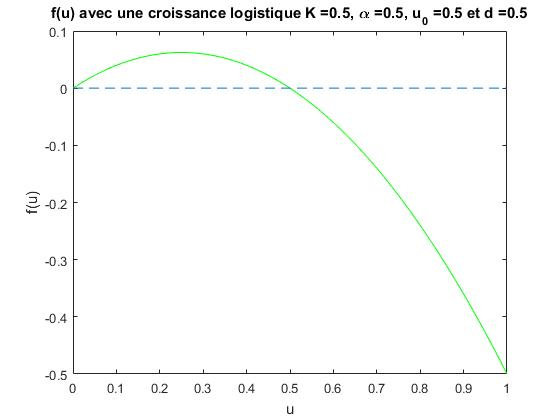
\includegraphics[width=0.45\linewidth]{SimulationKPP/figures1/fu}\hfill
	\caption{Fonction logistique de type KPP}
	\label{fu}
\end{figure}
\noindent
Le graphe de la figure \ref{fu} nous donne la représentation de la fonction logistique. 

\begin{figure}[H]
	\centering
	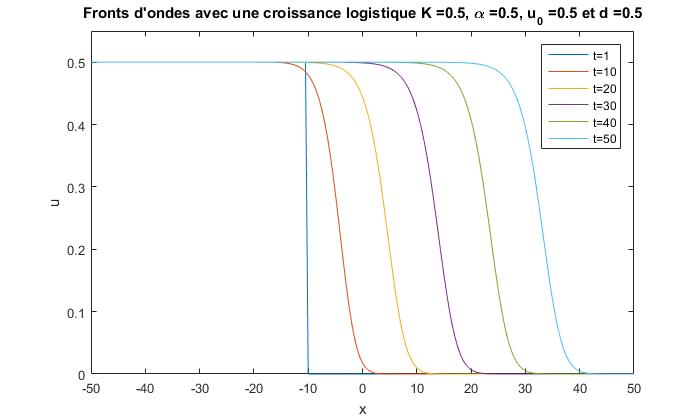
\includegraphics[width=0.55\linewidth]{SimulationKPP/figures1/FrontOnde2}\hfill
	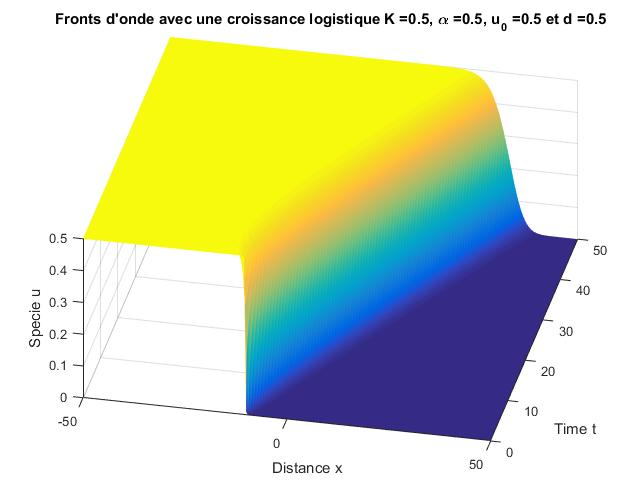
\includegraphics[width=0.40\linewidth]{SimulationKPP/figures1/FrontOnde1}\hfill
	\caption{Propagation du front d'onde en 1D}
\end{figure}
\noindent
On a pris ici comme condition initiale u$_0=0.5$ pour x < -10 et 0 ailleur.
On observe la propagation du front d'onde. Comme la condition initiale est égale à la capacité K, la taille de la population reste constante. On voit qu'une fois le front d'onde formé, la forme du front d'onde reste la même et progresse à une vitesse c>0.  

\subsubsection{Simulation de l'effet "hair trigger"}
\paragraph{Cas 1.1 : d=0.5, K=0.5, $\alpha =0.5$, $u_0=0.1$}

\begin{figure}[H]
	\centering
	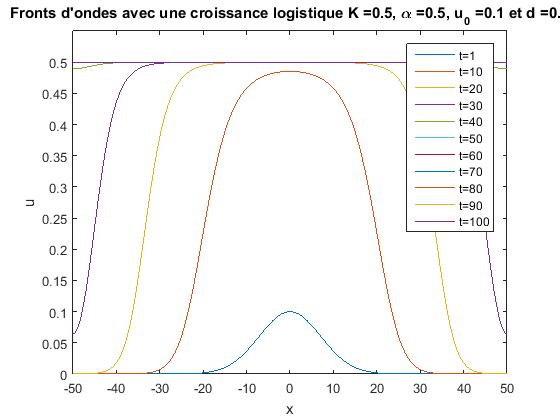
\includegraphics[width=0.45\linewidth]{SimulationKPP/TrigerEffect/fronts}\hfill
	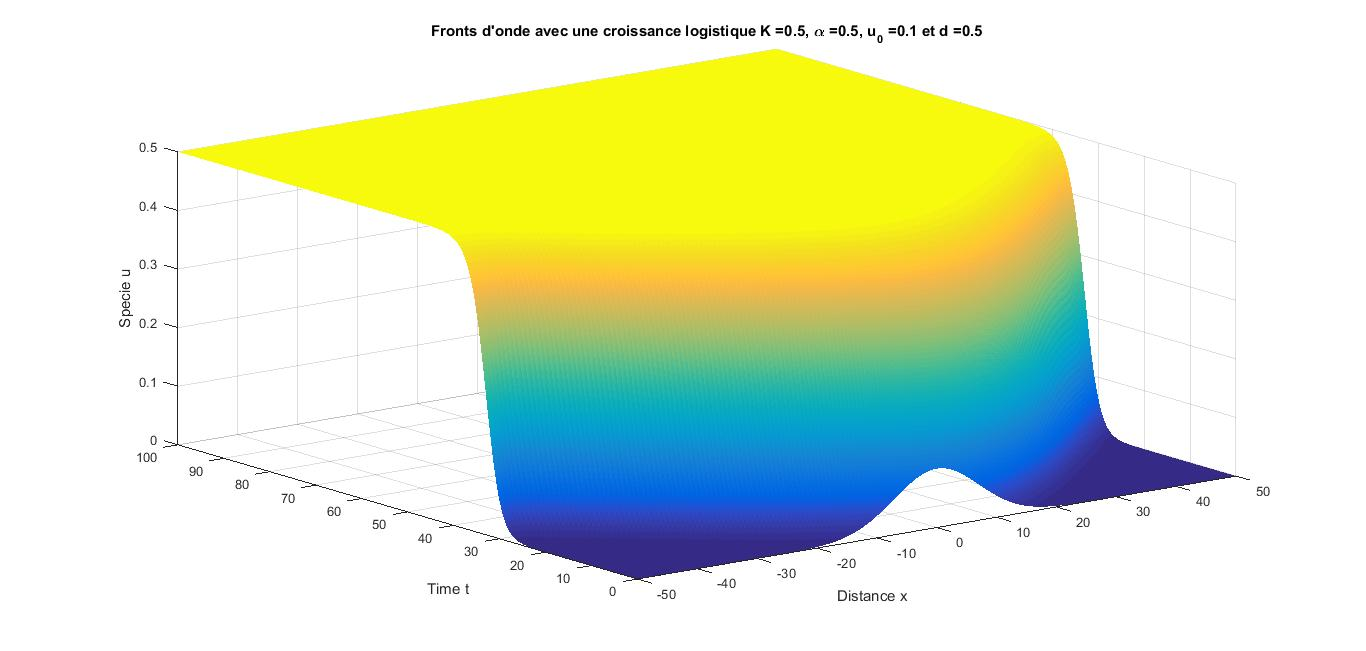
\includegraphics[width=0.55\linewidth]{SimulationKPP/TrigerEffect/Surf}\hfill
	\caption{Propagation du front d'onde en 1D avec une petite perturbation initiale}
\end{figure}
\noindent
On observe qu'avec une toute petite condition initiale, la population augmente et tend vers l'équilibre K.  


\begin{figure}[H]
	\centering
	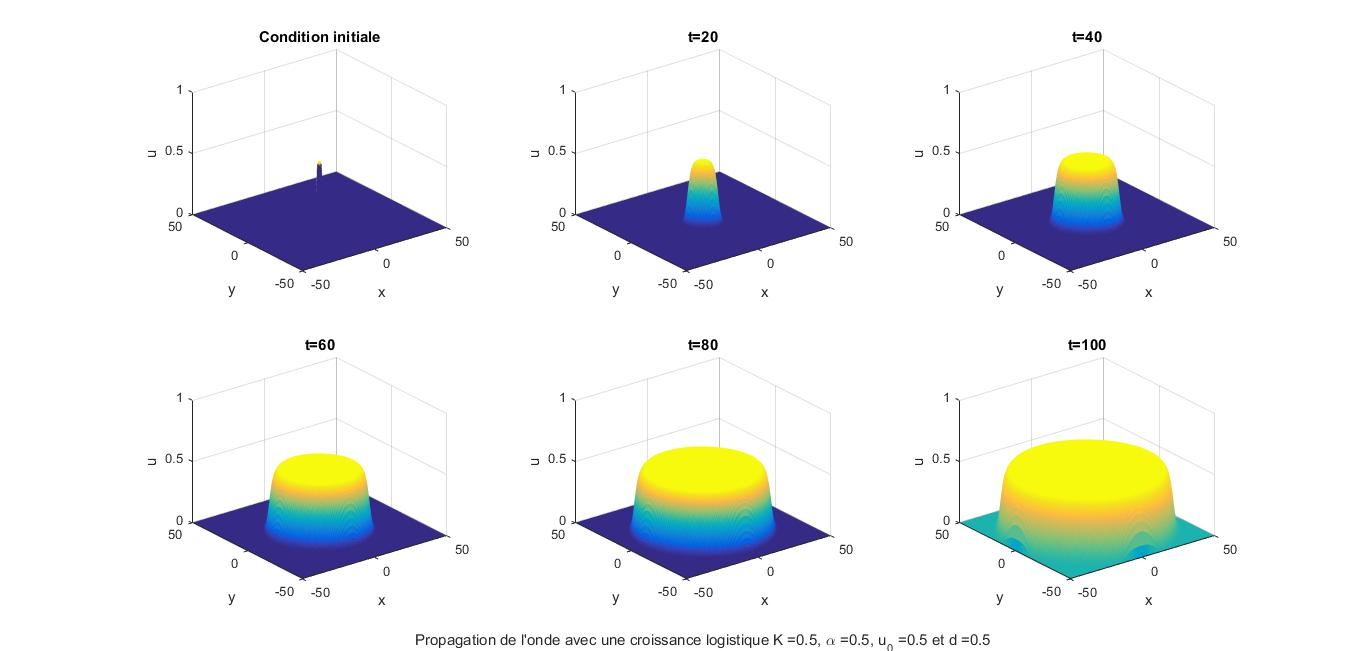
\includegraphics[width=1\linewidth]{SimulationKPP/KPP13}\hfill
    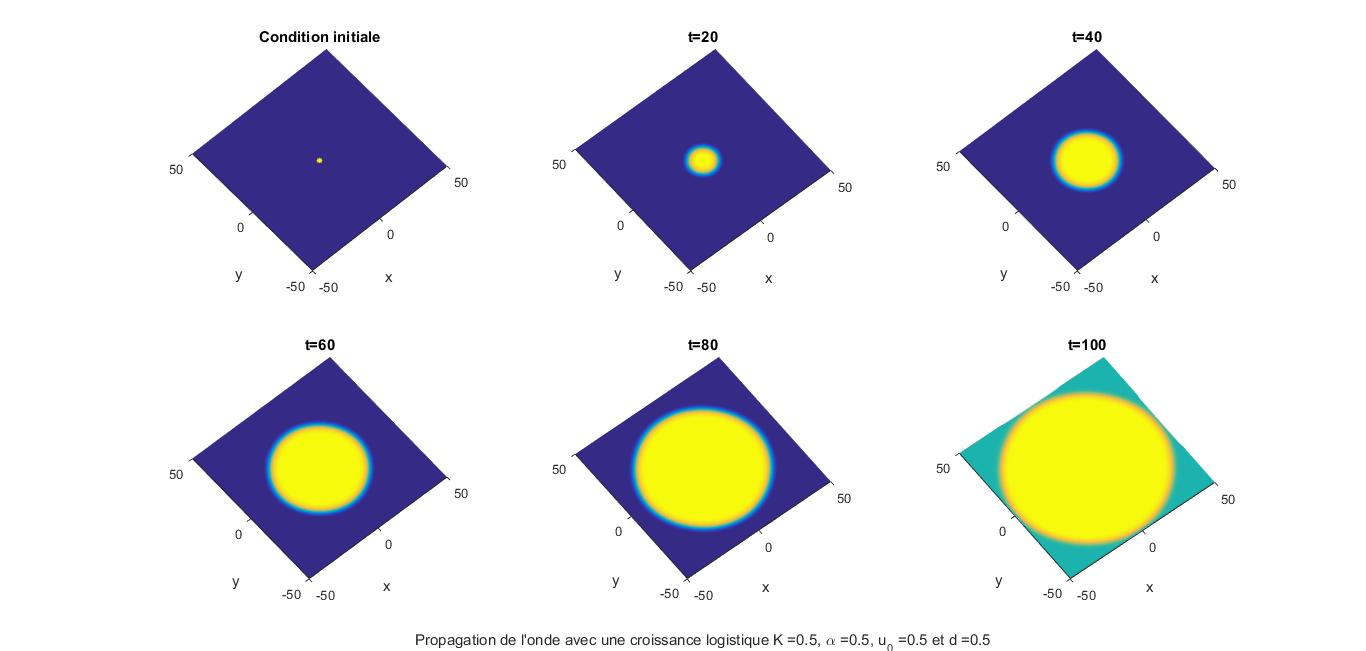
\includegraphics[width=1\linewidth]{SimulationKPP/KPP15}
    \caption{Propagation du front d'onde en 2D }
\end{figure}

On observe que la population grandit jusqu'à atteindre sa capacité maximale, et elle envahit l'espace.

\subsubsection{Effets de barrières ou variations géographiques }
On décide ici de modéliser des barrières géographiques tels que des montagnes ou le pôle nord qui pourrait avoir une influence sur la survie et la diffusion des population.
Pour cela on considère alors notre environnement comme hétérogène. On fait varier la capacité du milieu en fonction de la position dans l'espace.\\

\textbf{Effet d'une barrière géographique franchissable}
On décide de modéliser l'effet d'une barrière géographique franchissable comme une montagne. La montagne est représentée par la diagonale. Plus on s'éloigne de la diagonale, c'est à dire de la montagne, plus le coefficient K est élevé car les ressources y sont plus importantes. On initialise une petite population à droite de la montagne et on observe une évolution et une dispersion de la population sur les graphiques  \ref{Montagne} et \ref{MontagneBis} : 
\begin{figure}[H]
	\centering
	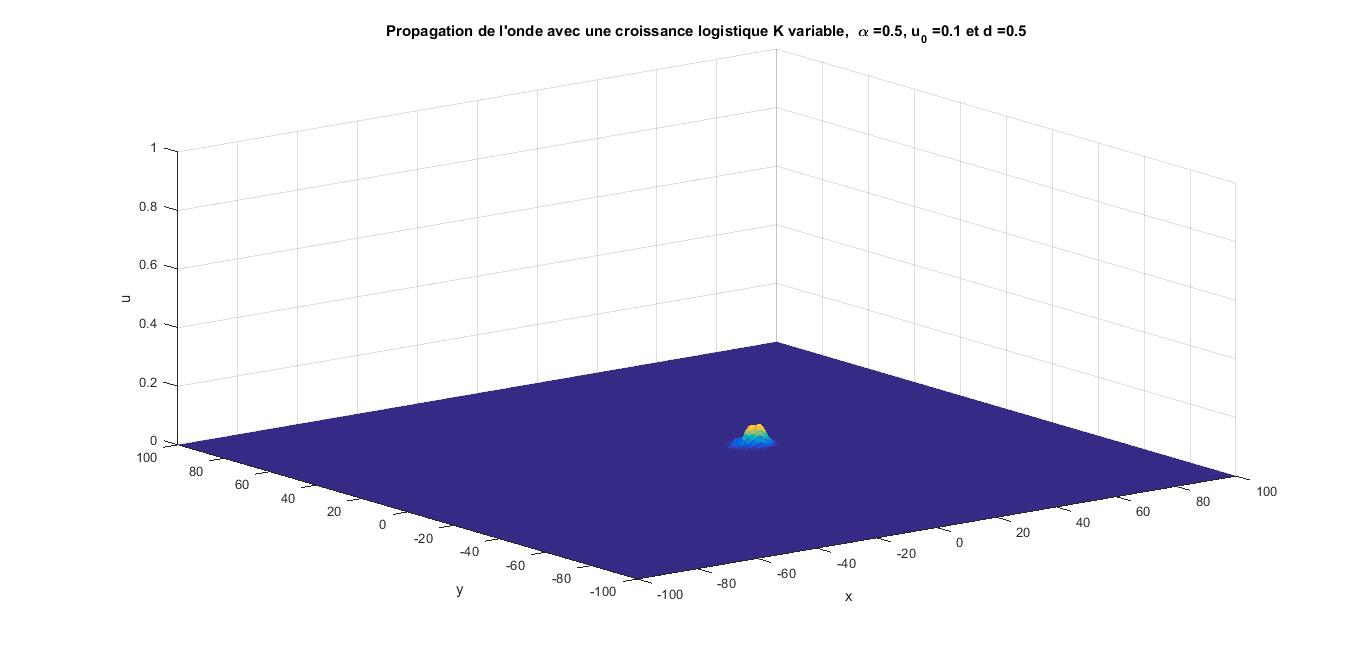
\includegraphics[width=0.5\linewidth]{SimulationKPP/Enviro/montagne1}\hfill
	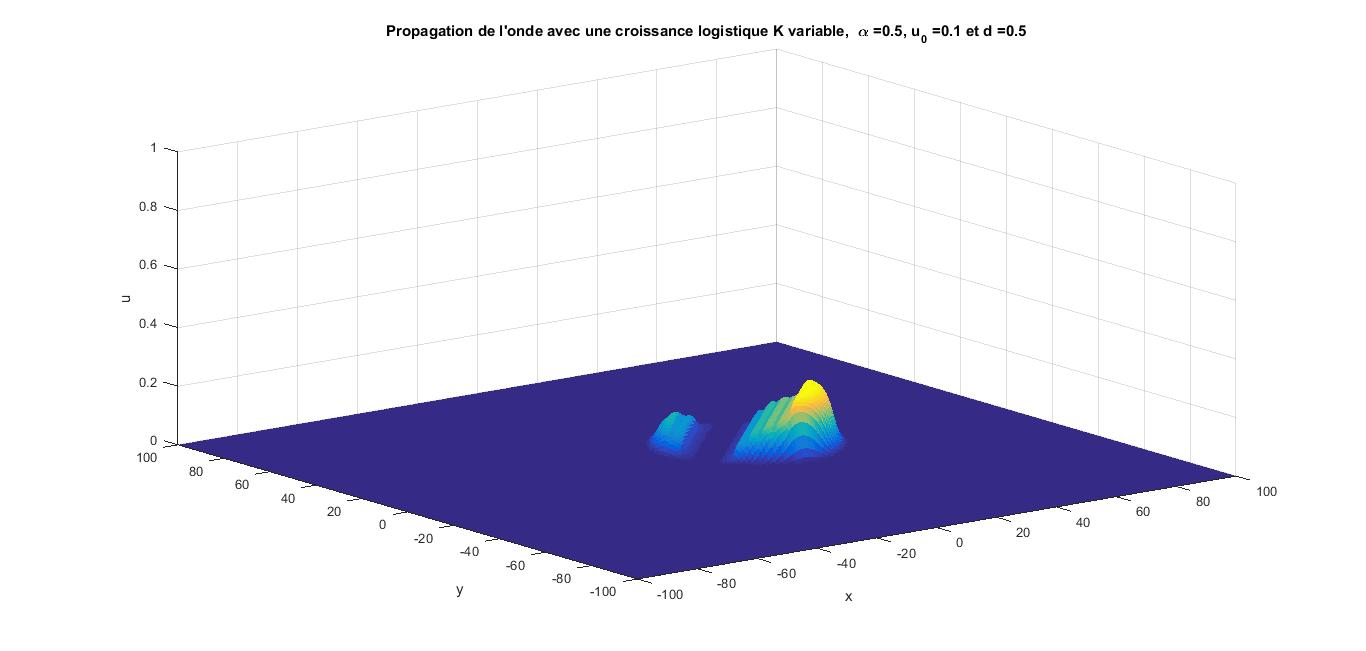
\includegraphics[width=0.5\linewidth]{SimulationKPP/Enviro/montagne3}\hfill
	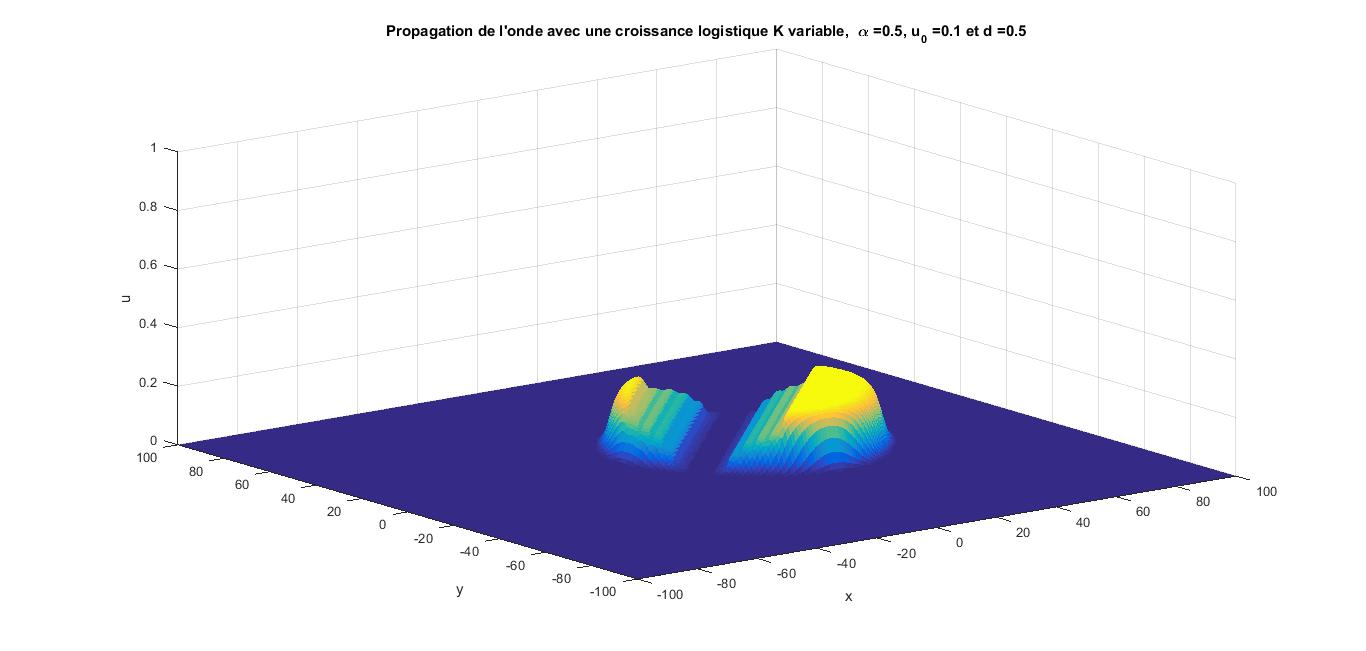
\includegraphics[width=0.5\linewidth]{SimulationKPP/Enviro/montagne5}\hfill
	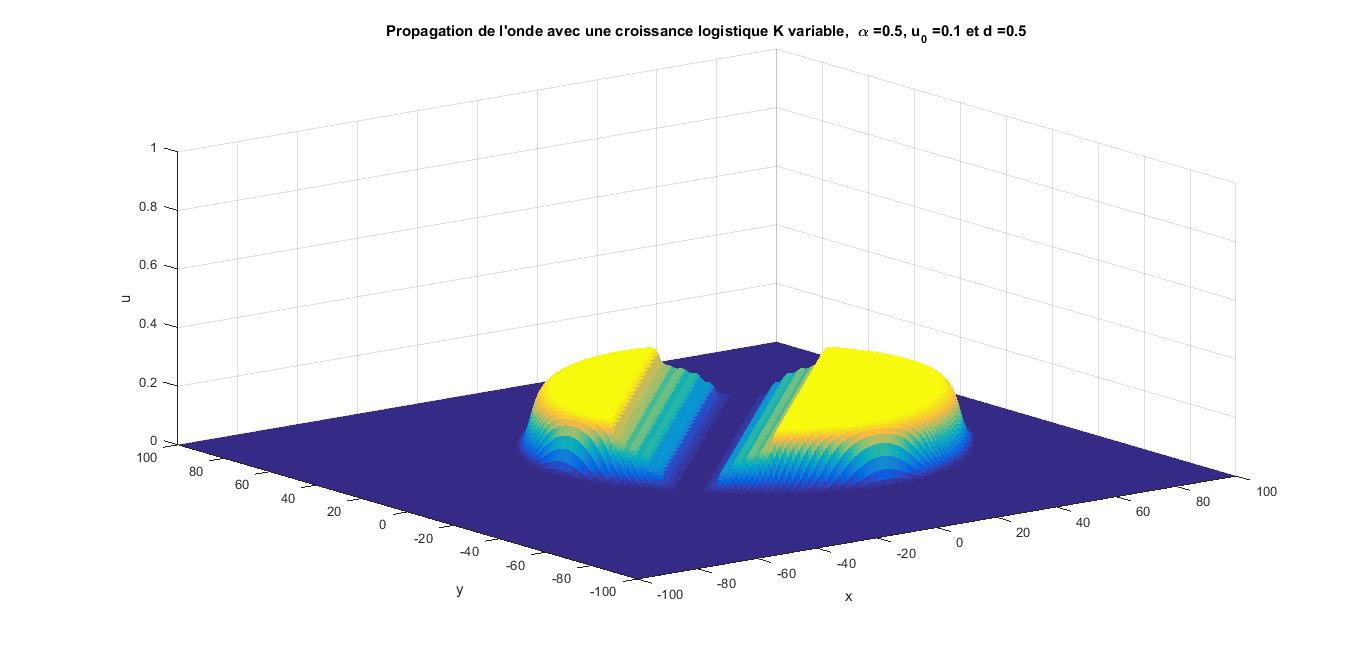
\includegraphics[width=0.5\linewidth]{SimulationKPP/Enviro/montagne8}
	\caption{Diffusion 2D de la population face à une montagne}
	\label{Montagne}
\end{figure}
\begin{figure}[H]
	\centering
	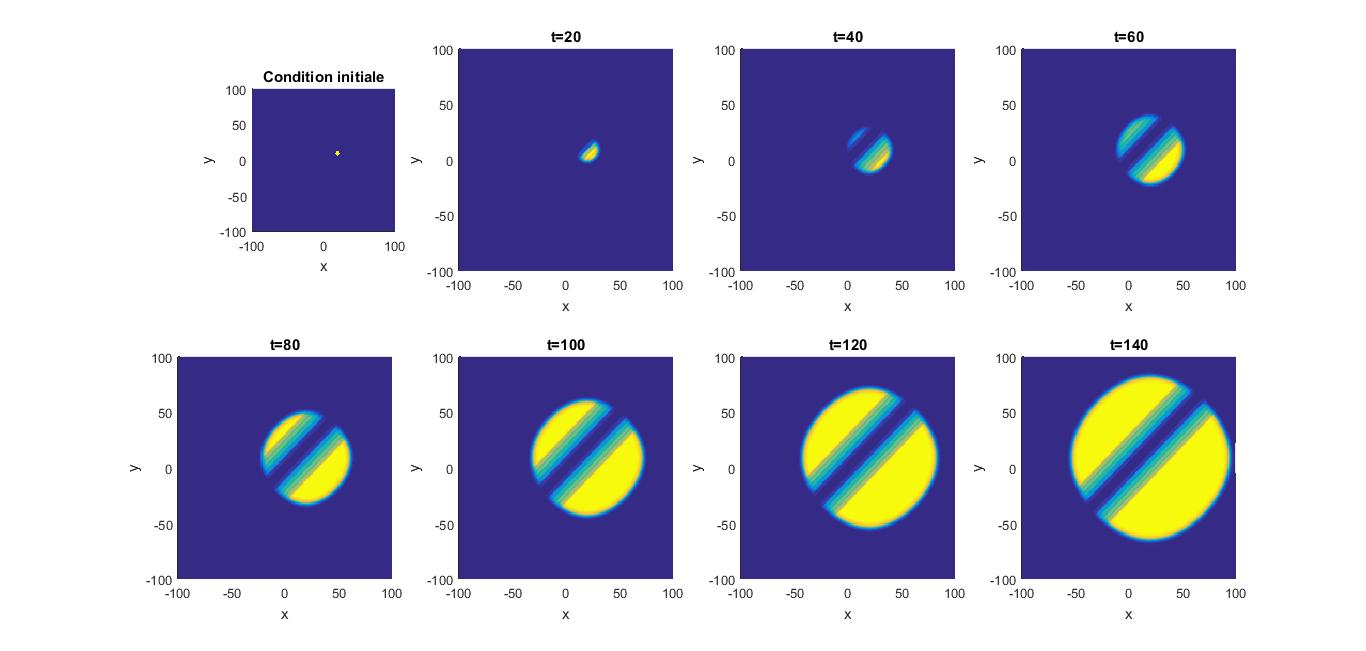
\includegraphics[width=0.7\linewidth]{SimulationKPP/Enviro/montagneVueHaut}
	\caption{Diffusion 2D de la population face à une montagne vue de haut}
	\label{MontagneBis}
\end{figure}

On observe que la présence de la montagne n'a pas d'effets sur la population, qui arrive à la dépasser pour rejoindre une autre zone. Une fois la population de l'autre côté elle arrive à croître sans problème.

<<<<<<< HEAD
\textbf{Effet d'une barrière géographique infranchissable}
On modélise ici par exemple un océan ou le pôle nord qui par un changement de climat entre les deux zones rend la vie impossible. En effet la température y est plus faible et les ressources moins importantes. En prend donc un K très petit sur une large zone, à gauche de la diagonale. 
=======
\textbf{Effet d'un changement de climat}
On modélise ici le changement de climat entre deux zones, par exemple avec le pôle nord où la température est plus faible et les ressources moins importantes. On prend donc un K très petit sur une large zone. 
>>>>>>> refs/remotes/origin/master

\begin{figure}[H]
	\centering
	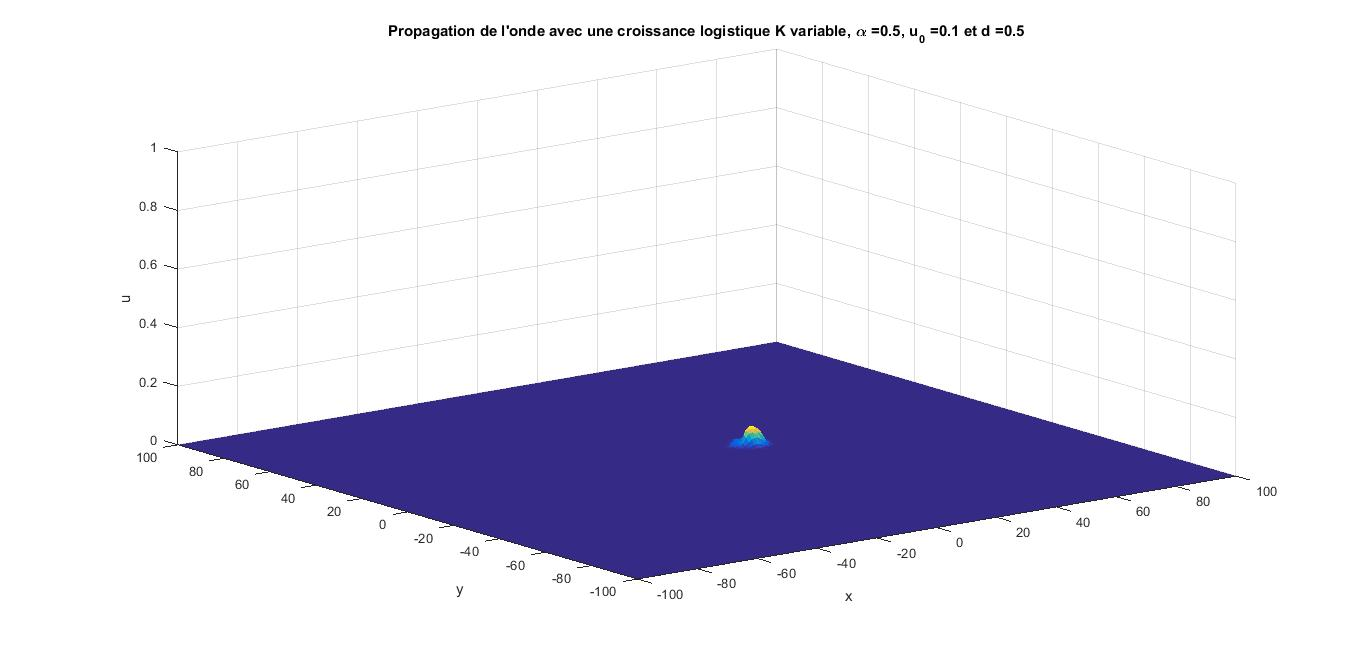
\includegraphics[width=0.5\linewidth]{SimulationKPP/Enviro/poleNord1}\hfill
	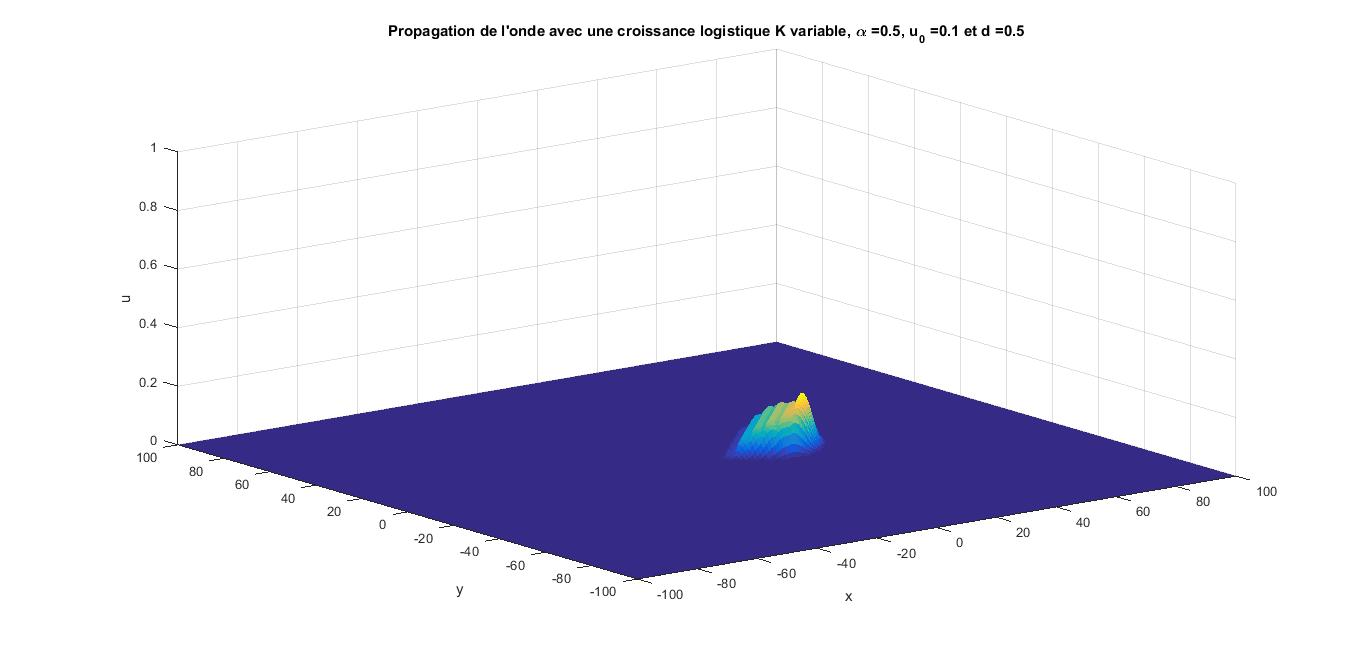
\includegraphics[width=0.5\linewidth]{SimulationKPP/Enviro/poleNord3}\hfill
	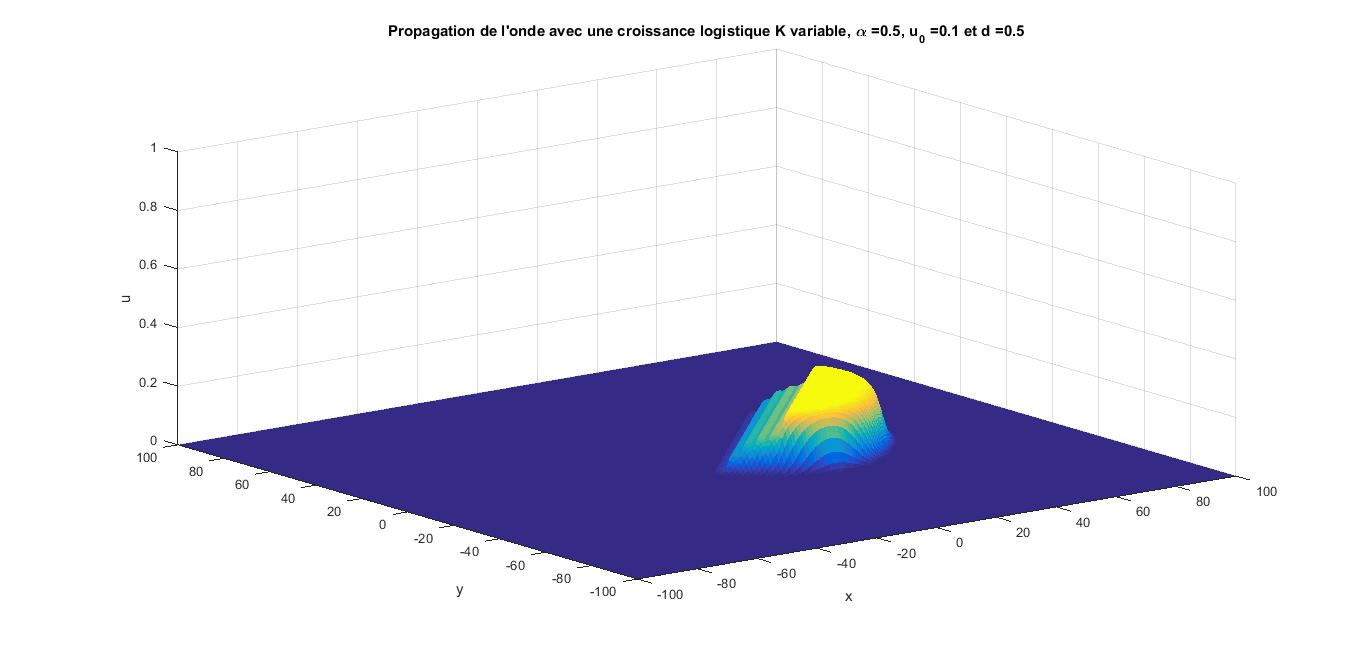
\includegraphics[width=0.5\linewidth]{SimulationKPP/Enviro/poleNord5}\hfill
	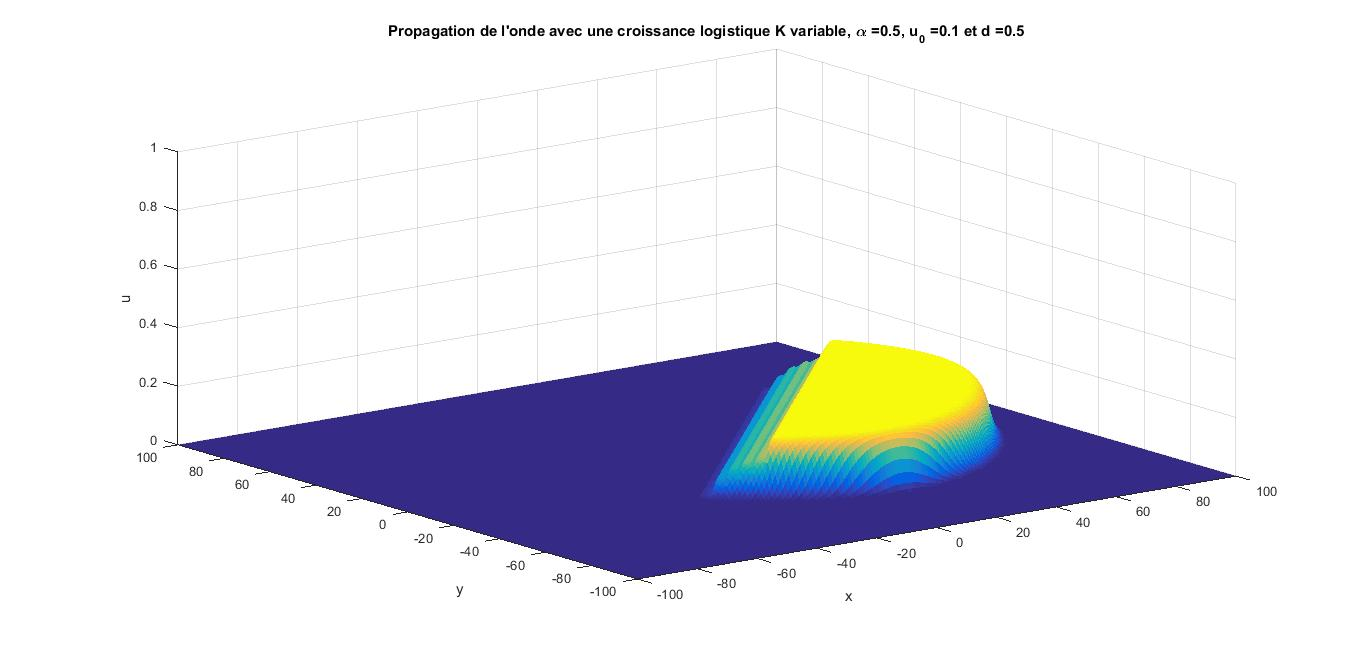
\includegraphics[width=0.5\linewidth]{SimulationKPP/Enviro/poleNord8}
	\caption{Diffusion 2D}
\end{figure}
\begin{figure}[H]
	\centering
	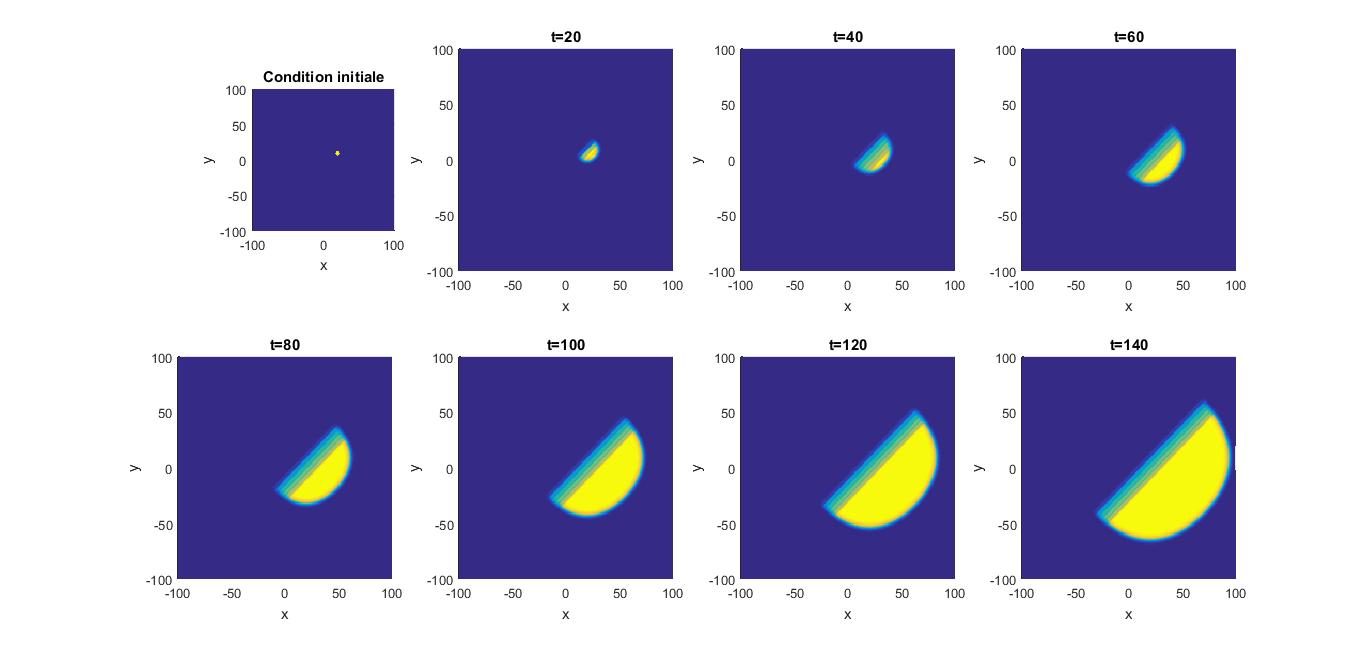
\includegraphics[width=0.7\linewidth]{SimulationKPP/Enviro/PolenordVueHaut}
	\caption{Diffusion 2D}
\end{figure}

On observe que la population se répend dans la zone où elle peut survivre.

Toutefois, on vois que le modèle de croissance logique ne prend pas en compte l'effet d'une toute petite population sur sa survie. 


<<<<<<< HEAD
=======
Toutefois, on vois que le modèle de croissance logistique ne prend pas en compte l'effet d'une toute petite population sur sa survie. 
>>>>>>> refs/remotes/origin/master
\subsection{Effet Allee}

\subsubsection{Constante de diffusion d=0.5}
On réalise une première série de simulations avec une constante de diffusion égale à 0.5 :
\paragraph{Cas 1.1 : $d=0.5, A=0.25 (k=64), u_0=0.1$}
\noindent
\begin{figure}[H]
	\centering
	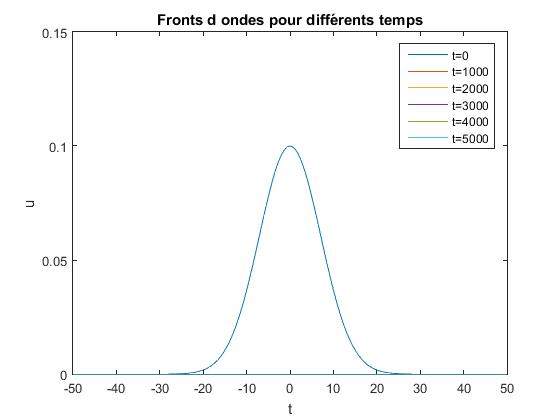
\includegraphics[width=0.40\linewidth]{Allee/F2311}\hfill
	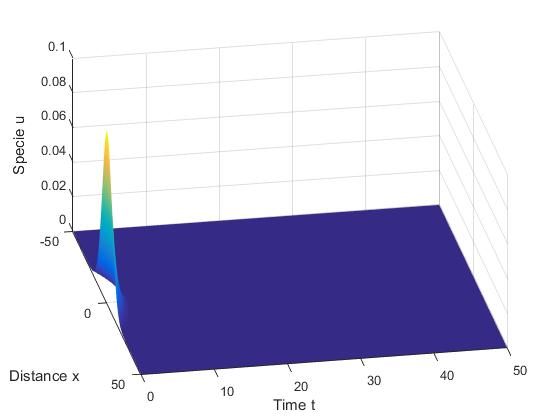
\includegraphics[width=0.55\linewidth]{Allee/F4311}
    \caption{Diffusion 1D}
\end{figure}
\noindent
\begin{figure}[H]
	\centering
	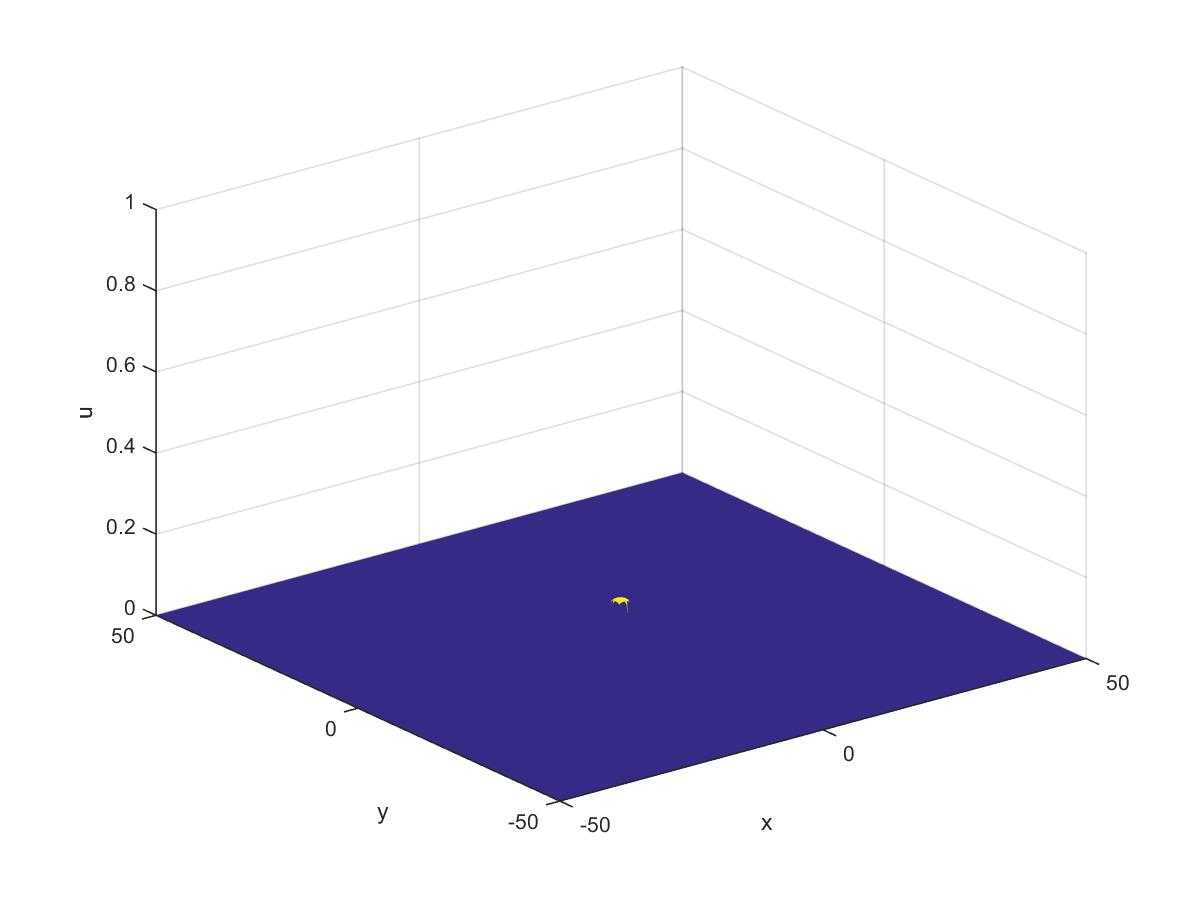
\includegraphics[width=0.3\linewidth]{Allee/311__1_}\hfill
    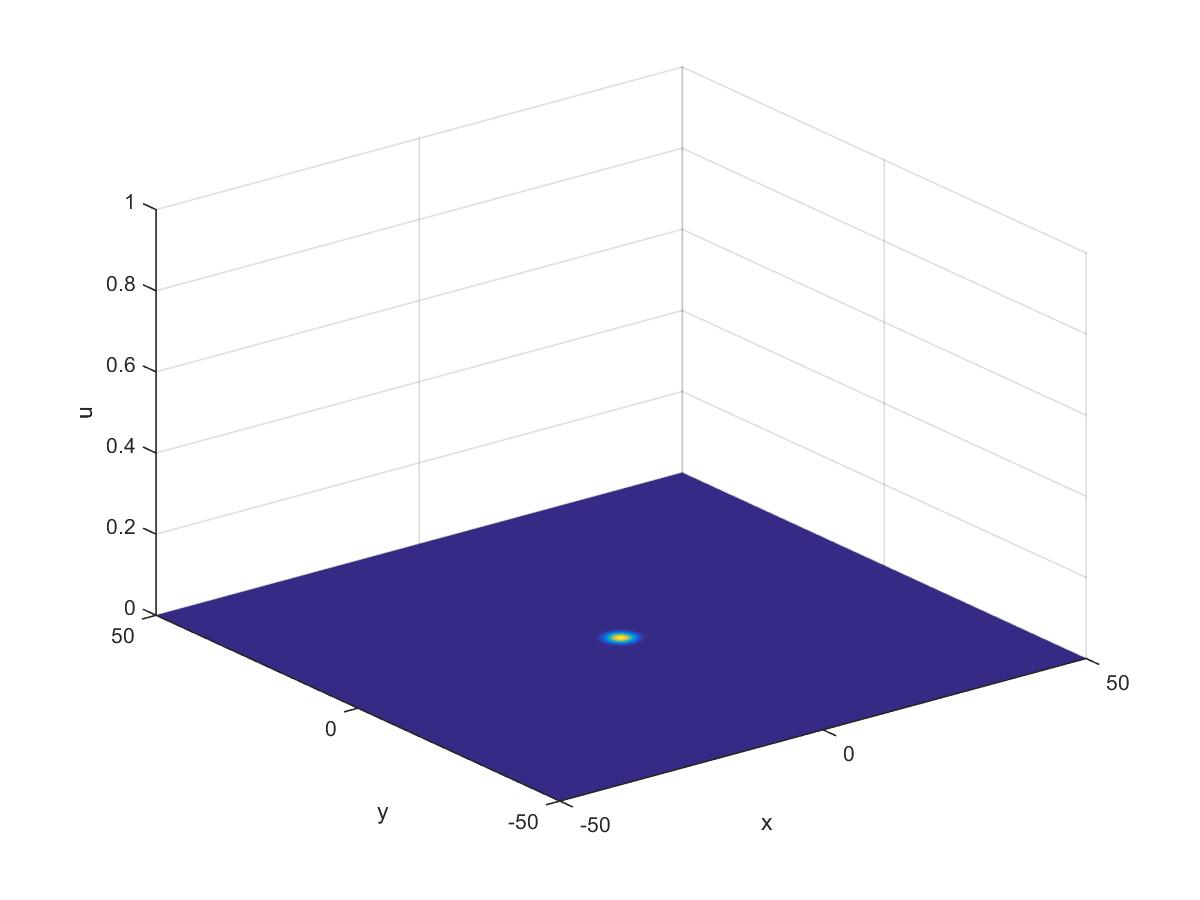
\includegraphics[width=0.3\linewidth]{Allee/311__2_}\hfill
	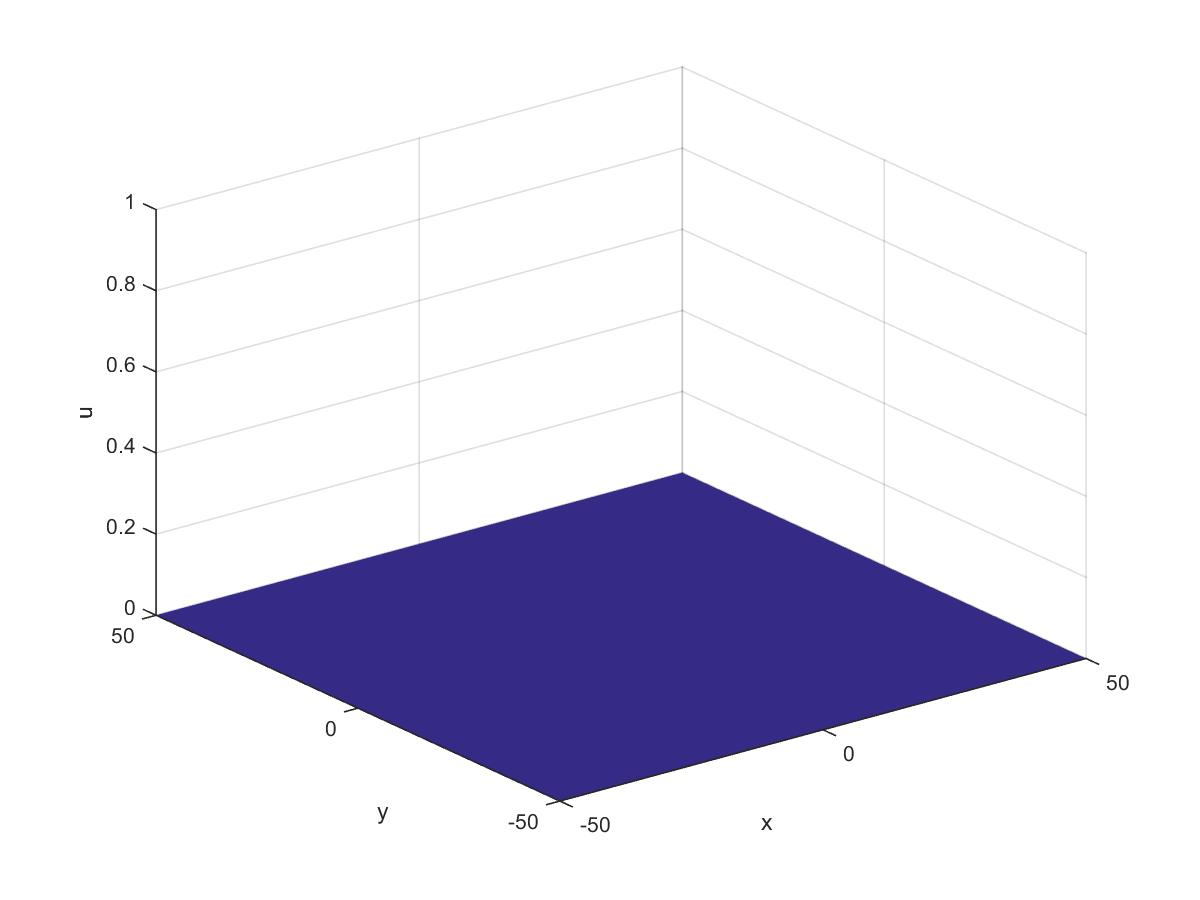
\includegraphics[width=0.3\linewidth]{Allee/311__3_}
    \caption{Diffusion 2D: t=0, t=500, t=5000}
\end{figure}
On se situe tout d'abord dans le cas où $A<0.5$. Comme montré dans l'étude analytique, on devrait avoir une vitesse positive et l'équilibre 1 devrait donc envahir l'équilibre 0. Toutefois, on a choisi une condition initiale $u_0<A$. On se situe donc dans le cas où la densité de population initiale est inférieure à la densité de population critique : le taux de croissance par individu devient donc négatif (c'est le principe de l'effet Allee fort). Malgré la diffusion, la population va donc rapidement s'éteindre.

\paragraph{Cas 1.2 : $d=0.5, A=0.25 (k=64), u_0=0.5$}
\noindent
\begin{figure}[H]
	\centering
	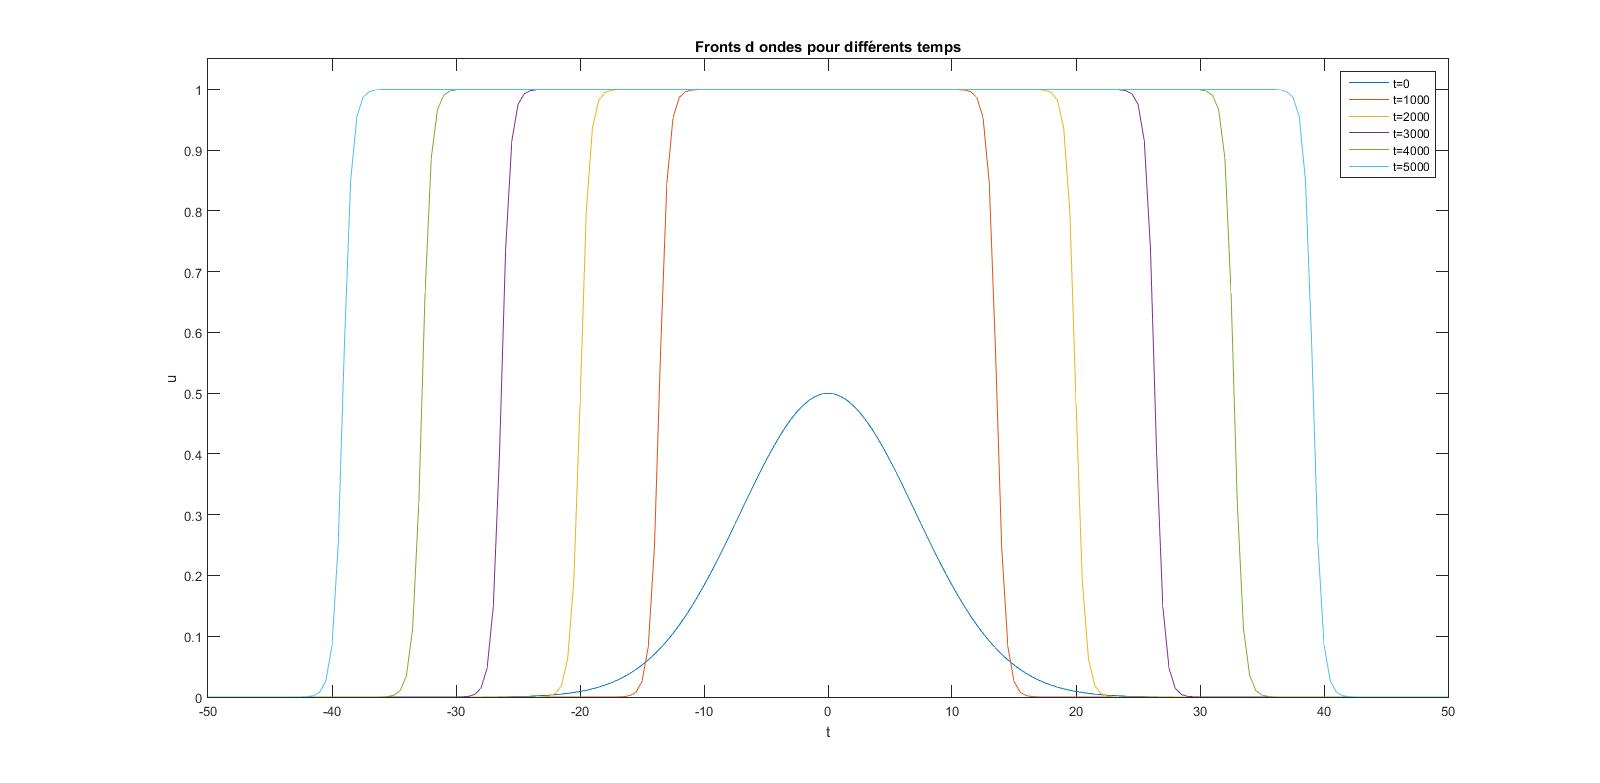
\includegraphics[width=0.40\linewidth]{Allee/F2312}\hfill
	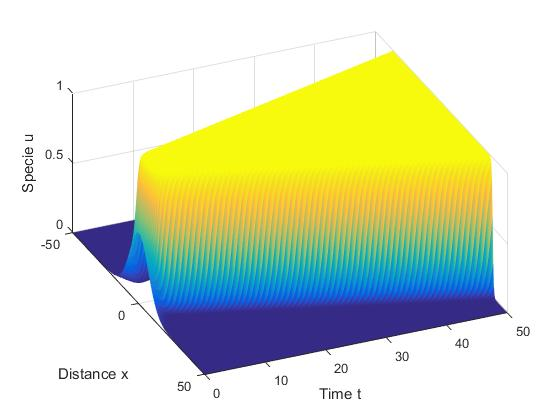
\includegraphics[width=0.55\linewidth]{Allee/F4312}
    \caption{Diffusion 1D}
    \label{3121}
\end{figure}
\noindent
\begin{figure}[H]
	\centering
	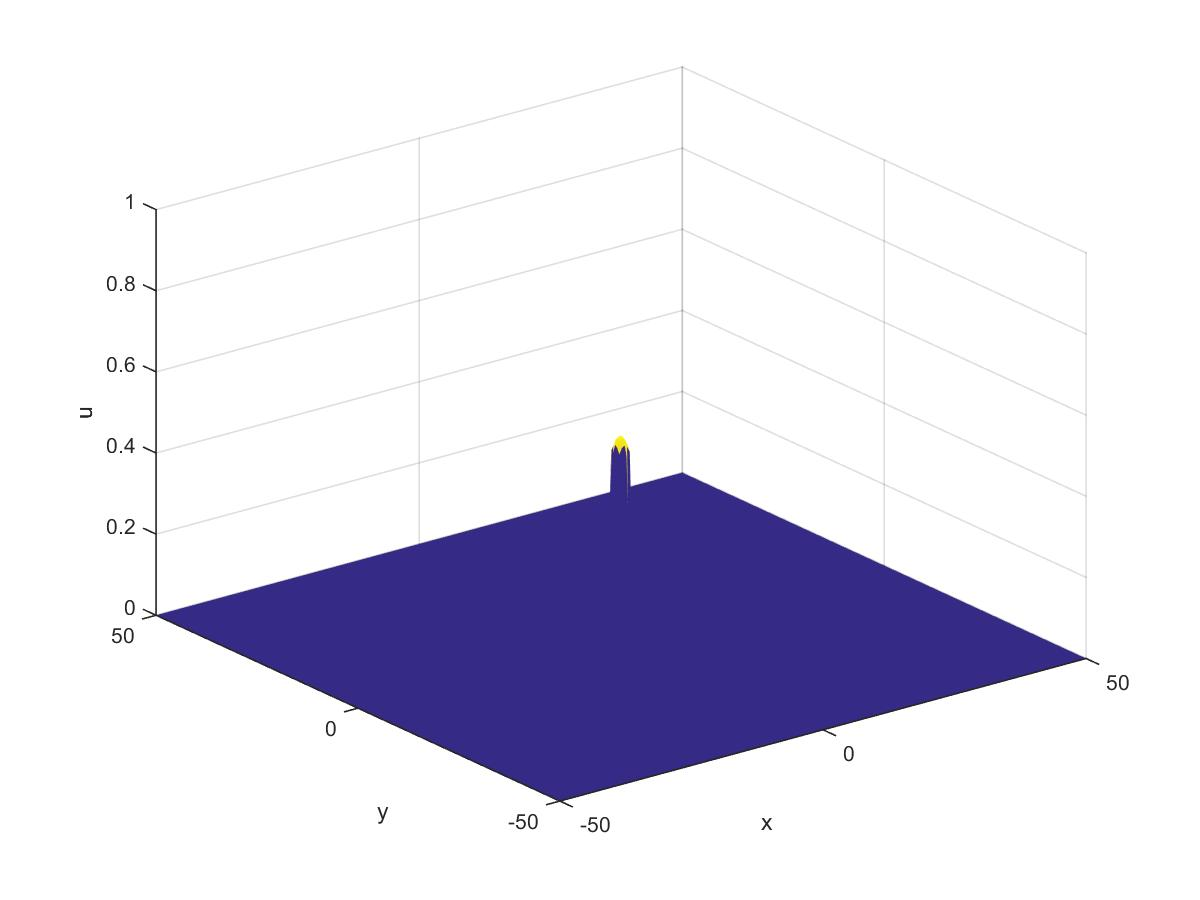
\includegraphics[width=0.3\linewidth]{Allee/312__1_}\hfill
    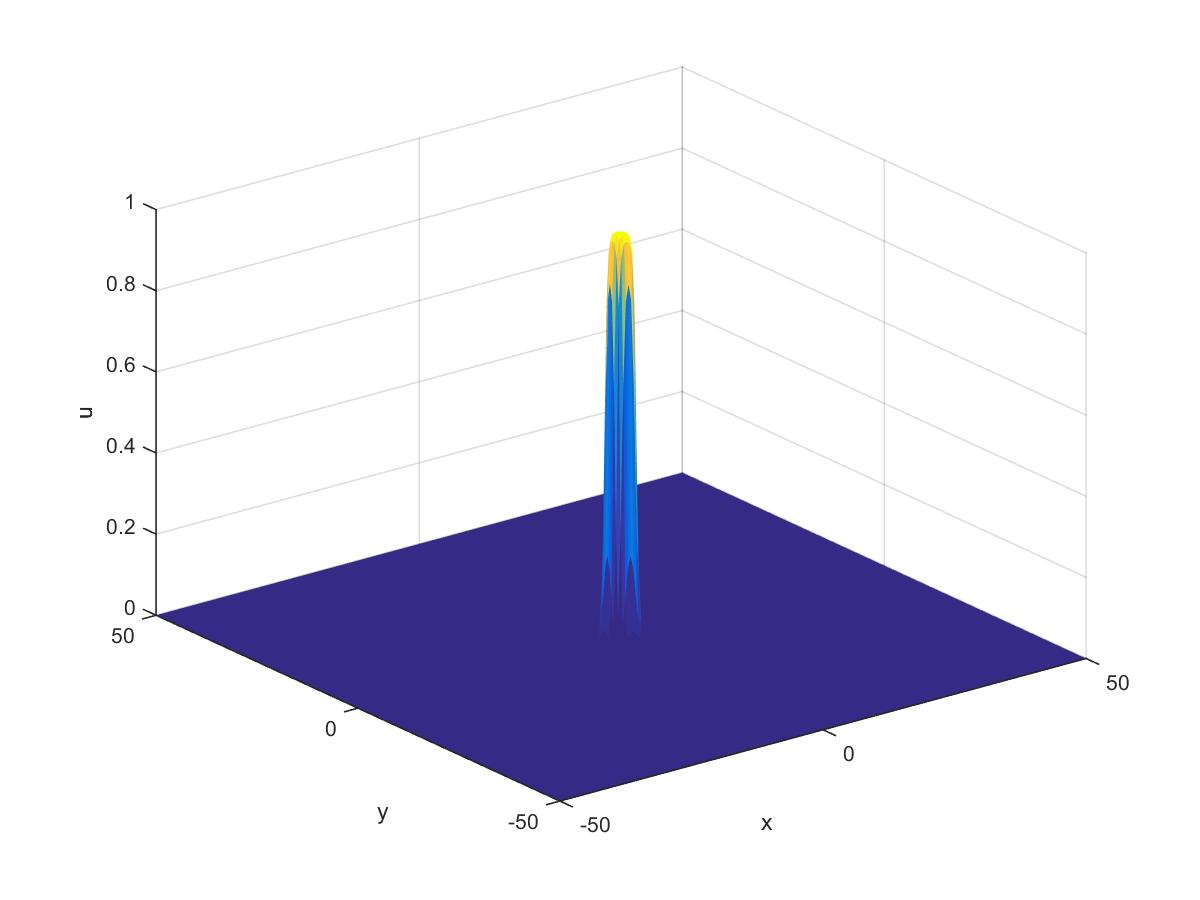
\includegraphics[width=0.3\linewidth]{Allee/312__2_}\hfill
	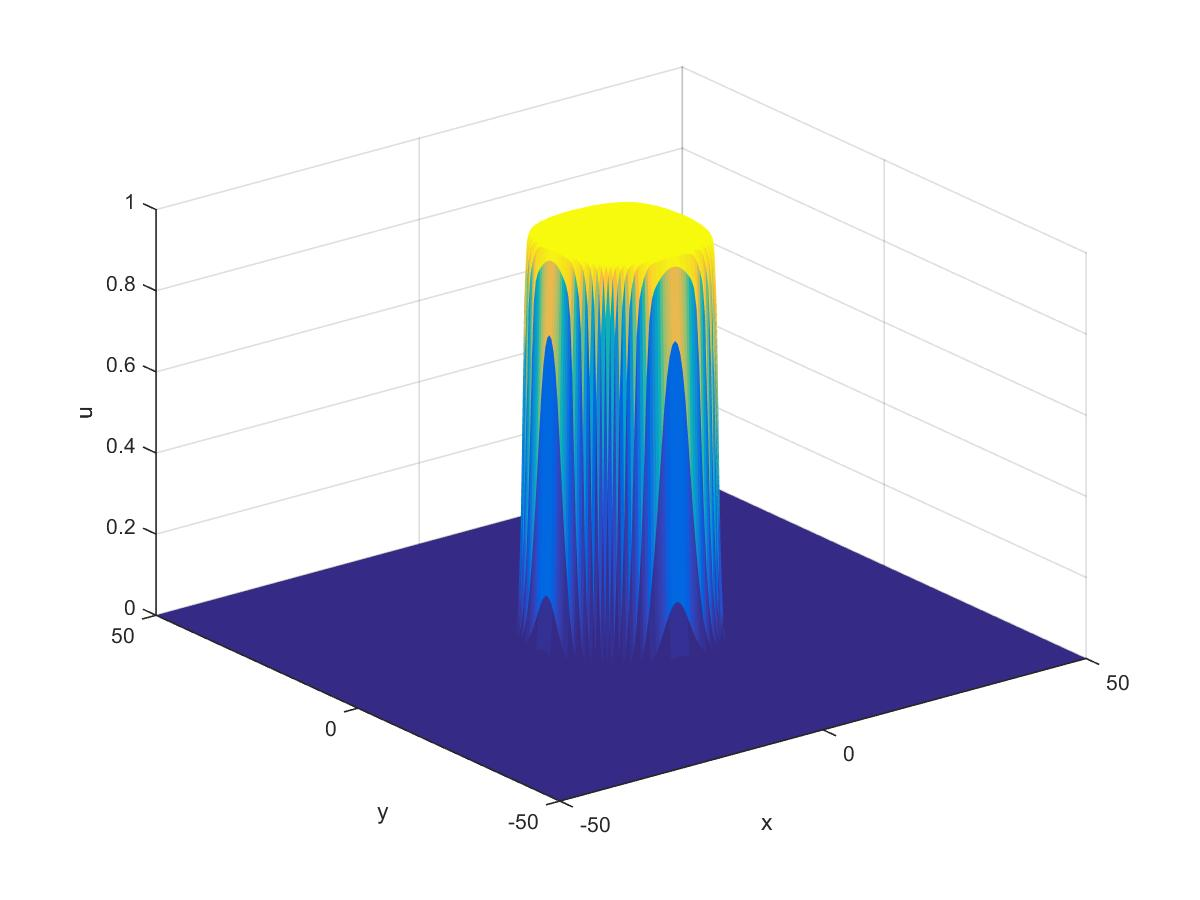
\includegraphics[width=0.3\linewidth]{Allee/312__3_}
    \caption{Diffusion 2D: t=0, t=500, t=5000}
    \label{3122}
\end{figure}
On se situe maintenant toujours dans le cas où $A<0.5$, mais cette fois avec $u_0>A$. On a toujours une vitesse positive qui implique que l'état d'équilibre 1 envahisse l'état d'équilibre 0. La densité initiale n'étant pas inférieure à la densité critique, le taux de croissance est positif et l'état d'équilibre 1 va donc être rapidement atteint et va ensuite diffuser sur l'ensemble de l'espace. C'est bien ce que l'on peut observer, tant en une dimension (figure \ref{3121}) qu'en deux dimension (figure \ref{3122}). On observe d'abord une hausse de la population locale avant qu'elle ne diffuse en envahisse progressivement tout l'espace.

\paragraph{Cas 1.3 : $d=0.5, A=0.75 (k=7.1), u_0=0.5$}
\noindent
\begin{figure}[H]
	\centering
	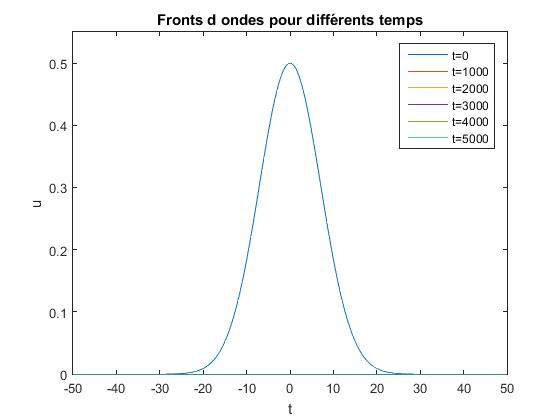
\includegraphics[width=0.40\linewidth]{Allee/F2322}\hfill
	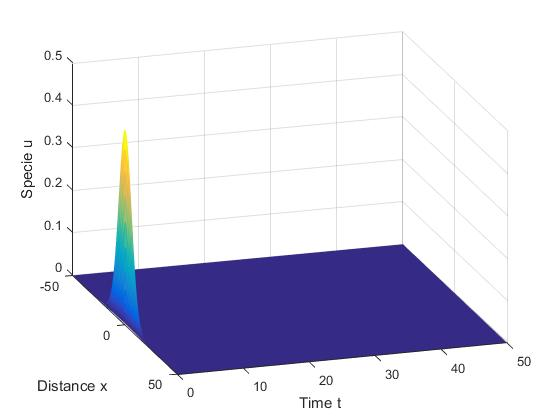
\includegraphics[width=0.55\linewidth]{Allee/F4322}
    \caption{Diffusion 1D}
\end{figure}
\noindent
\begin{figure}[H]
	\centering
	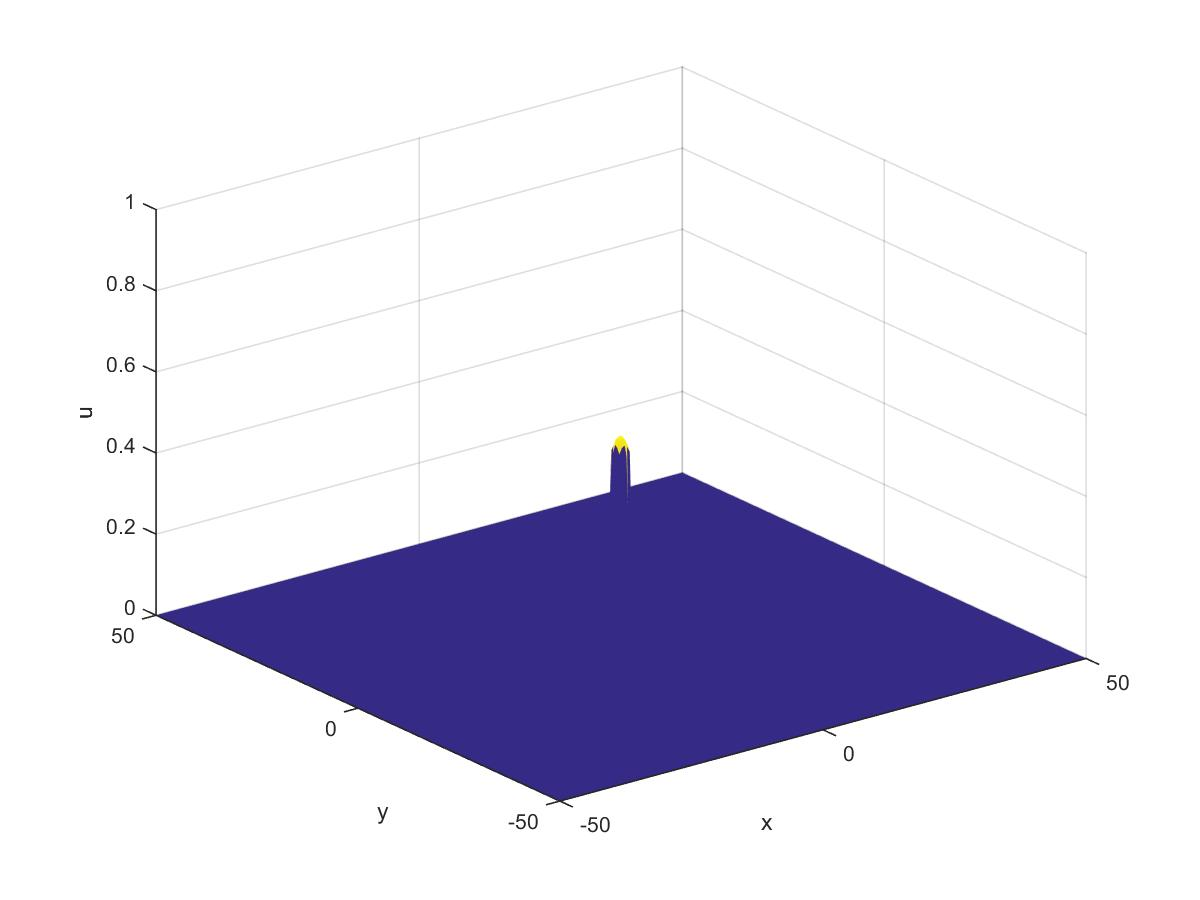
\includegraphics[width=0.3\linewidth]{Allee/322__1_}\hfill
    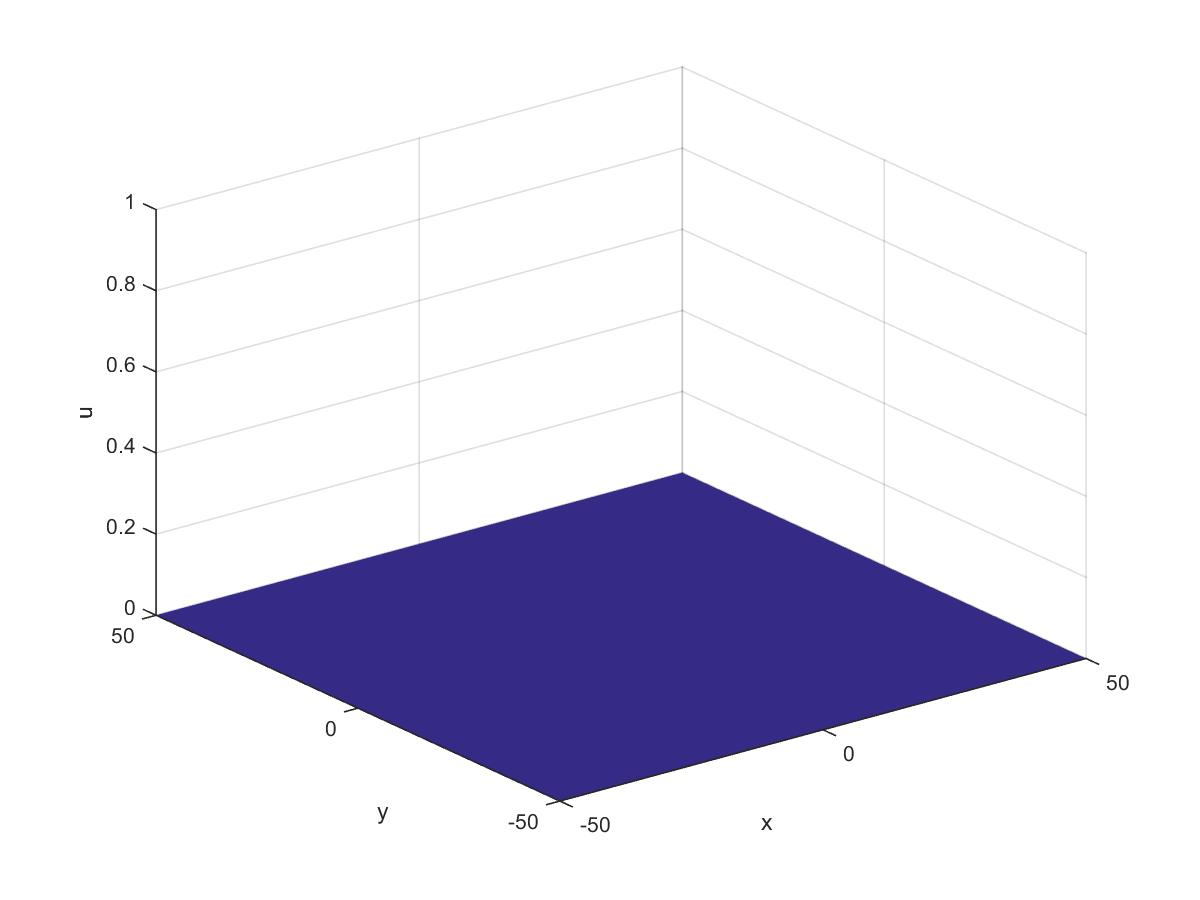
\includegraphics[width=0.3\linewidth]{Allee/322__2_}\hfill
	\includegraphics[width=0.3\linewidth]{Allee/{322__3_}}
    \caption{Diffusion 2D: t=0, t=500, t=5000}
\end{figure}
On se situe tout maintenant dans le cas où $A>0.5$. Comme montré dans l'étude analytique, on devrait avoir une vitesse négative et l'équilibre 0 devrait donc envahir l'équilibre 1. De plus, on a choisi une condition initiale $u_0<A$. On se situe là encore dans le cas où le taux de croissance par individu devient négatif ce qui induit que la population va donc rapidement s'éteindre. Ce phénomène est d'autant plus rapide que dans le cas 1.1 puisque la vitesse de diffusion est négative.

\paragraph{Cas 1.4 : $d=0.5, A=0.75 (k=7.1), u_0=0.9$}
\noindent
\begin{figure}[H]
	\centering
	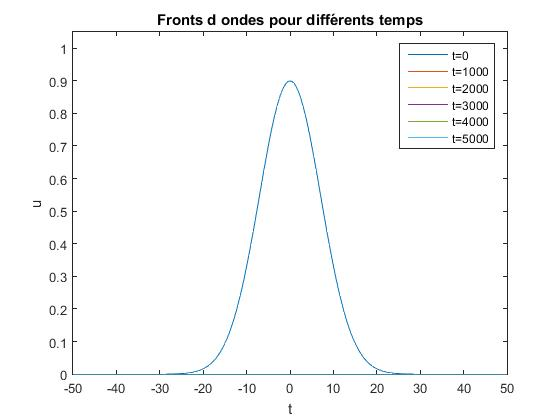
\includegraphics[width=0.40\linewidth]{Allee/F2323}\hfill
	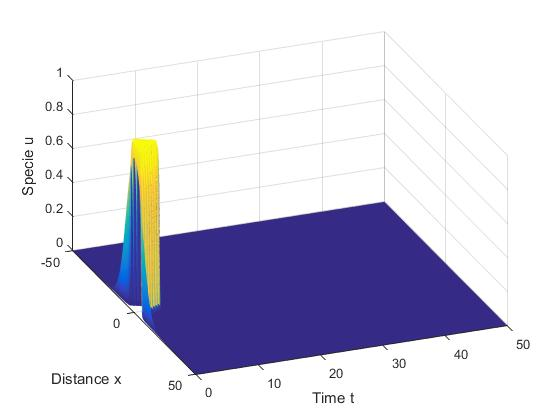
\includegraphics[width=0.55\linewidth]{Allee/F4323}
    \caption{Diffusion 1D}
\end{figure}
\noindent
\begin{figure}[H]
	\centering
	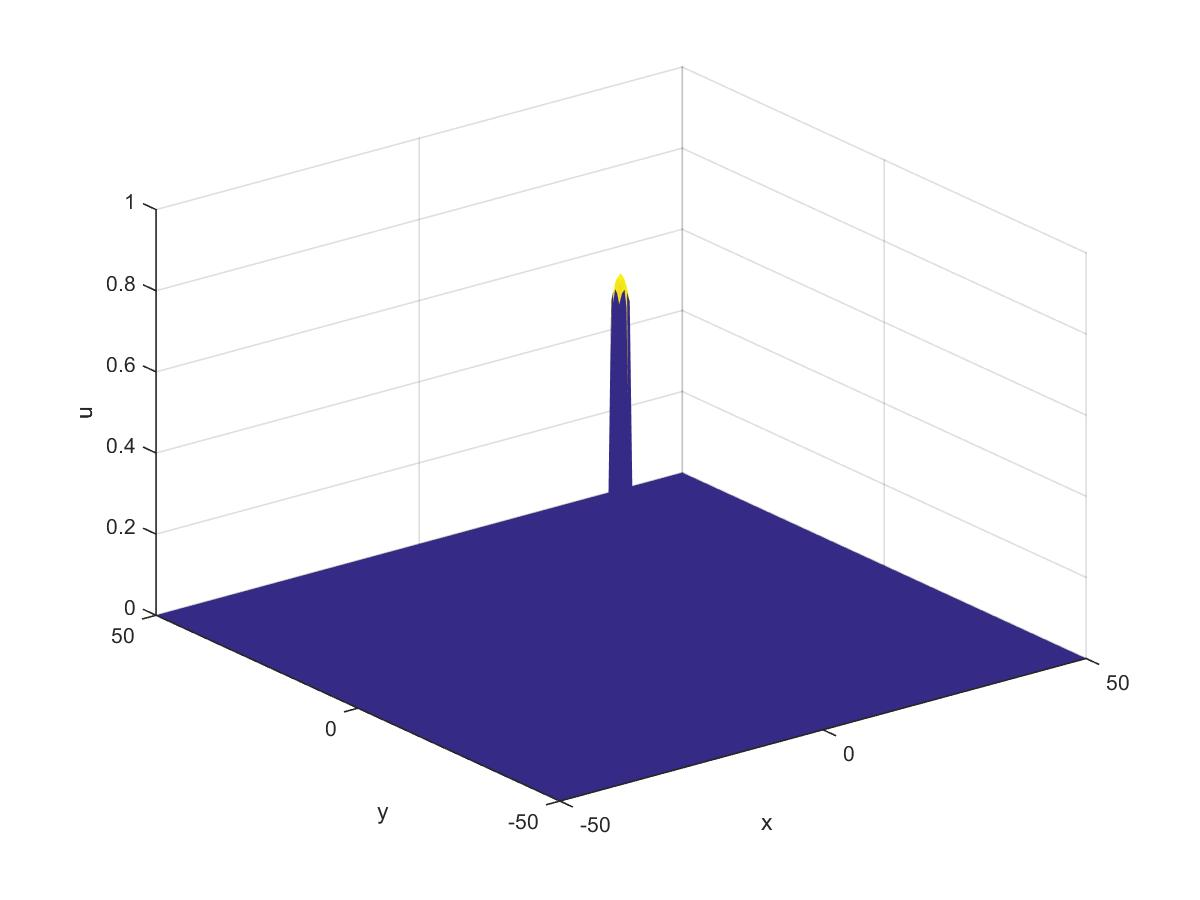
\includegraphics[width=0.3\linewidth]{Allee/323__1_}\hfill
    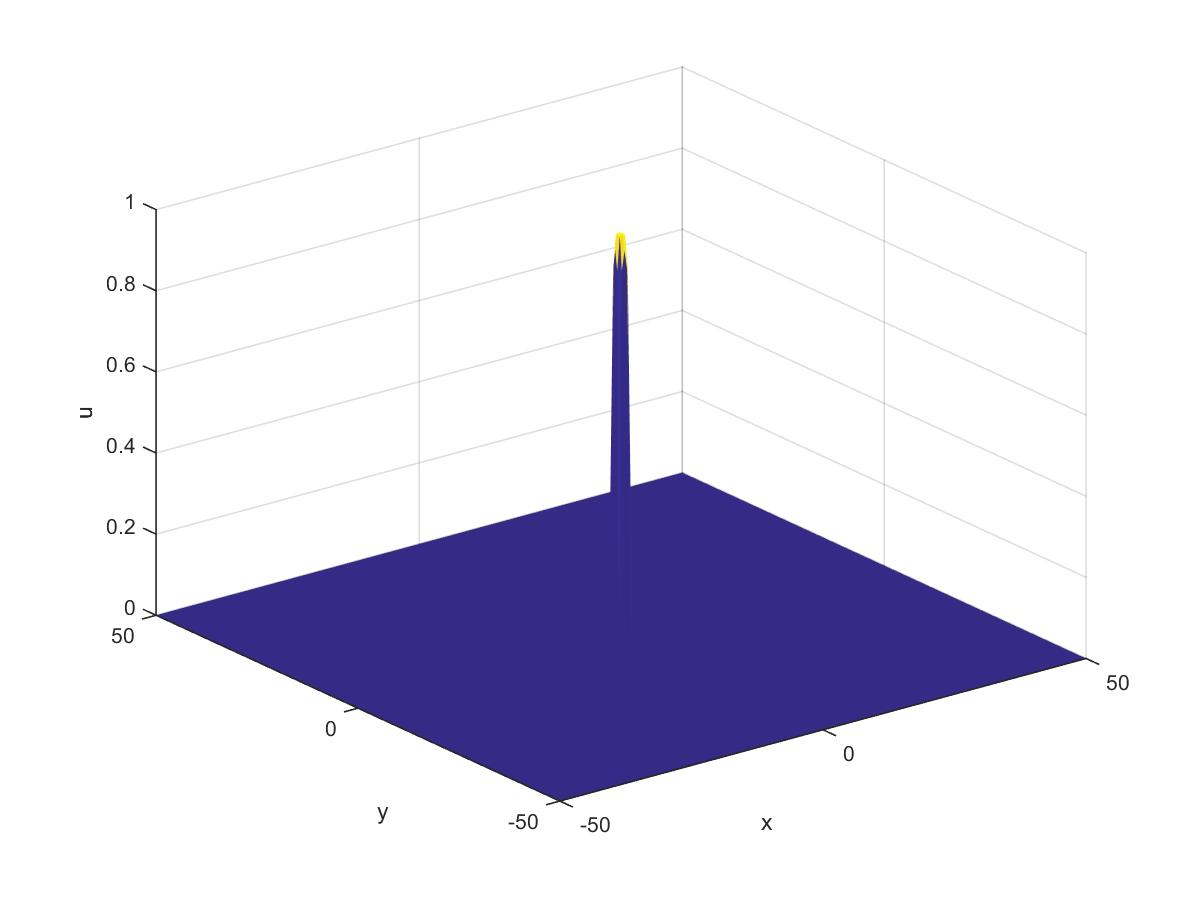
\includegraphics[width=0.3\linewidth]{Allee/323__2_}\hfill
	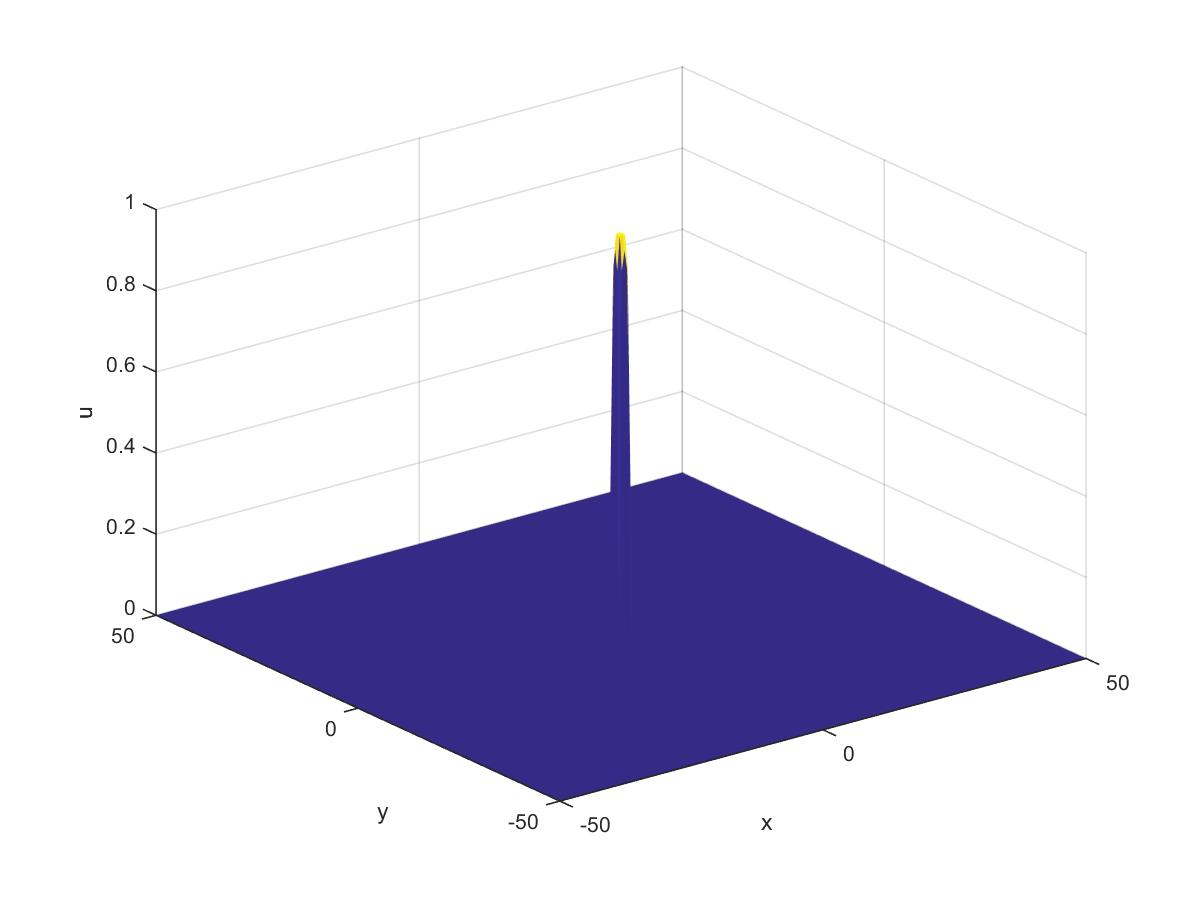
\includegraphics[width=0.3\linewidth]{Allee/323__3_}
    \caption{Diffusion 2D: t=0, t=500, t=5000}
\end{figure}
On se situe encore dans le cas où $A>0.5$. On a donc encore une vitesse négative et l'équilibre 0 devrait donc envahir l'équilibre 1. On a  cette fois choisi une condition initiale $u_0>A$. On peut donc observer dans un premier temps une hausse de la densité de population qui tend vers l'équilibre 1. Toutefois, la vitesse négative de la diffusion induit peu à peu la disparition de l'espèce dont le territoire conquis est peu à peu retreint jusqu'à être nul.

\paragraph{Cas 1.5 : $d=0.5, A=0.5 (k=16), u_0=0.1$}
\noindent
\begin{figure}[H]
	\centering
	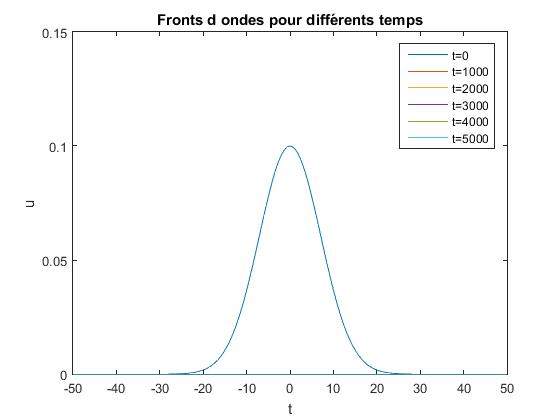
\includegraphics[width=0.40\linewidth]{Allee/F2331}\hfill
	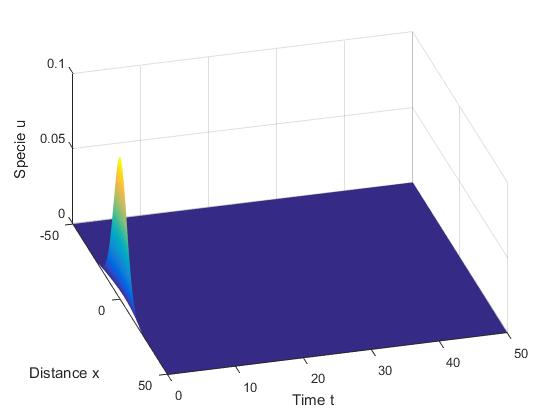
\includegraphics[width=0.55\linewidth]{Allee/F4331}
    \caption{Diffusion 1D}
\end{figure}
\noindent
\begin{figure}[H]
	\centering
	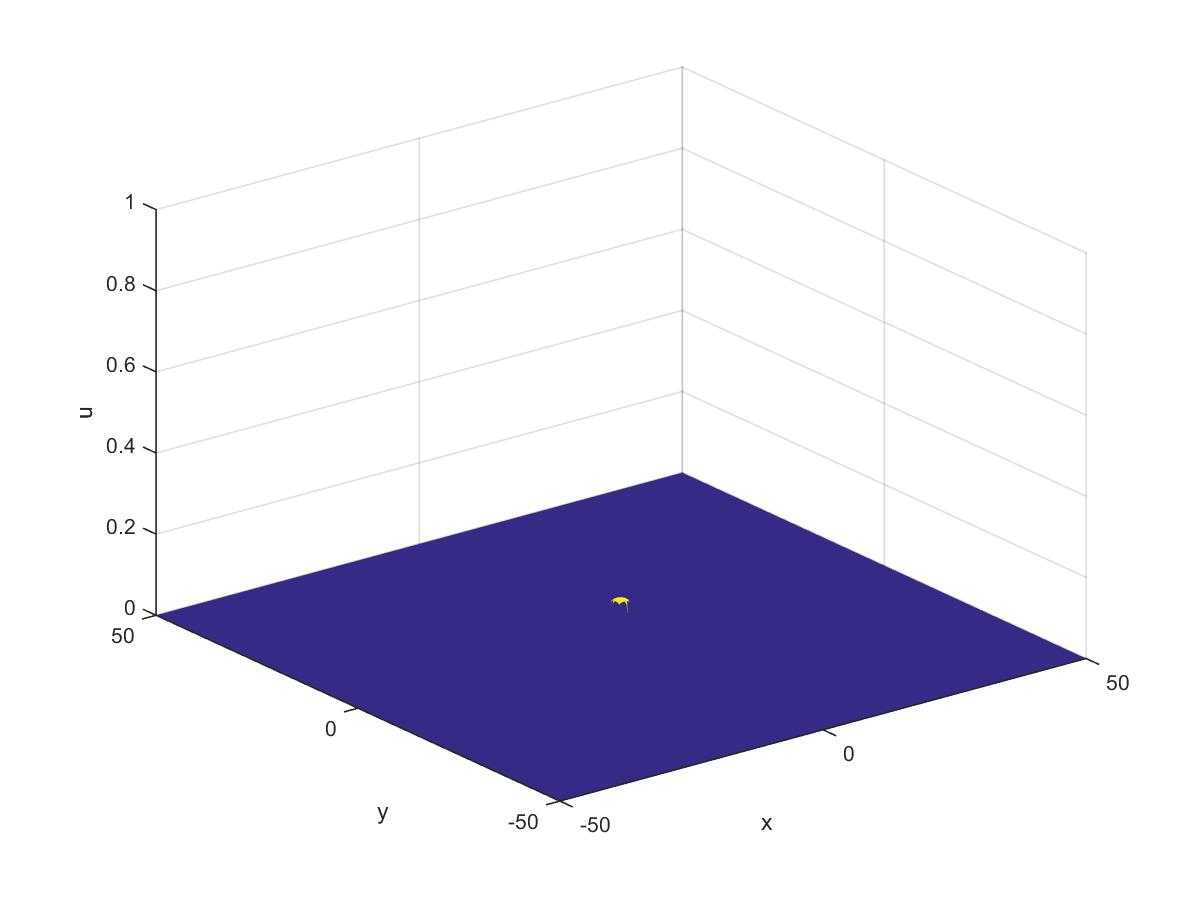
\includegraphics[width=0.3\linewidth]{Allee/331__1_}\hfill
    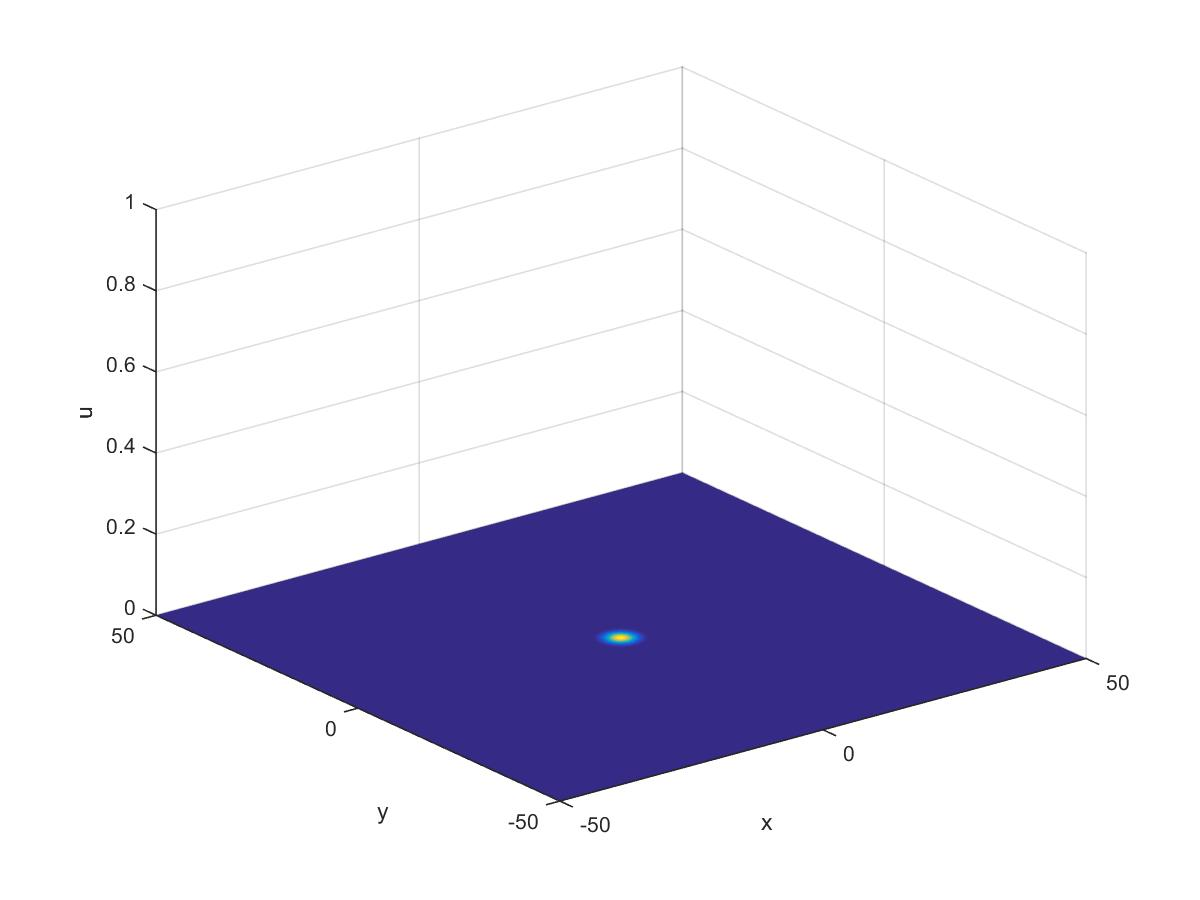
\includegraphics[width=0.3\linewidth]{Allee/331__2_}\hfill
	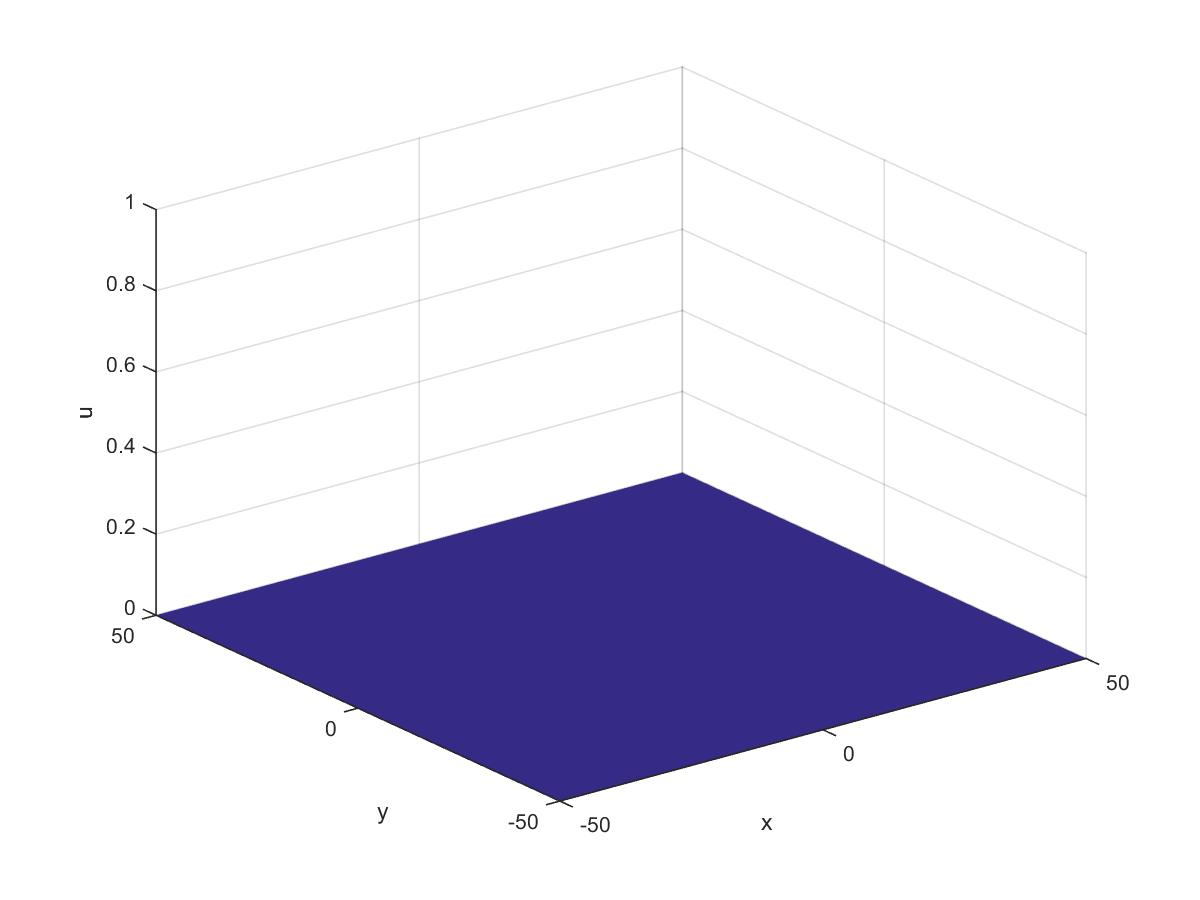
\includegraphics[width=0.3\linewidth]{Allee/331__3_}
    \caption{Diffusion 2D: t=0, t=500, t=5000}
\end{figure}
On se situe dans le cas très particulier où $A=0.5$. On devrait donc avoir une vitesse de diffusion nulle. ici, on a choisi une condition initiale $u_0<A$. Le phénomène Allee va donc s'appliquer et la population va rapidement tendre à l'extinction.

\paragraph{Cas 1.6 : $d=0.5, A=0.5 (k=16), u_0=0.9$}
\noindent
\begin{figure}[H]
	\centering
	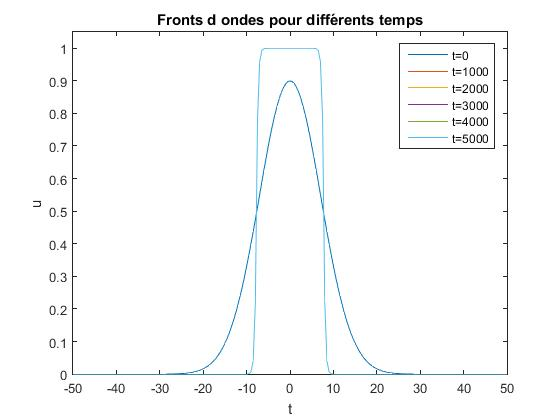
\includegraphics[width=0.40\linewidth]{Allee/F2333}\hfill
	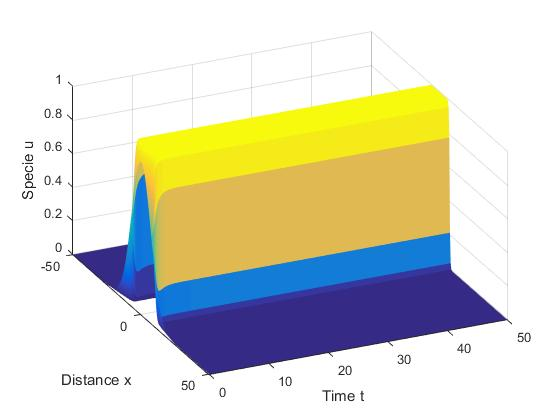
\includegraphics[width=0.55\linewidth]{Allee/F4333}
    \caption{Diffusion 1D}
\end{figure}
\noindent
\begin{figure}[H]
	\centering
	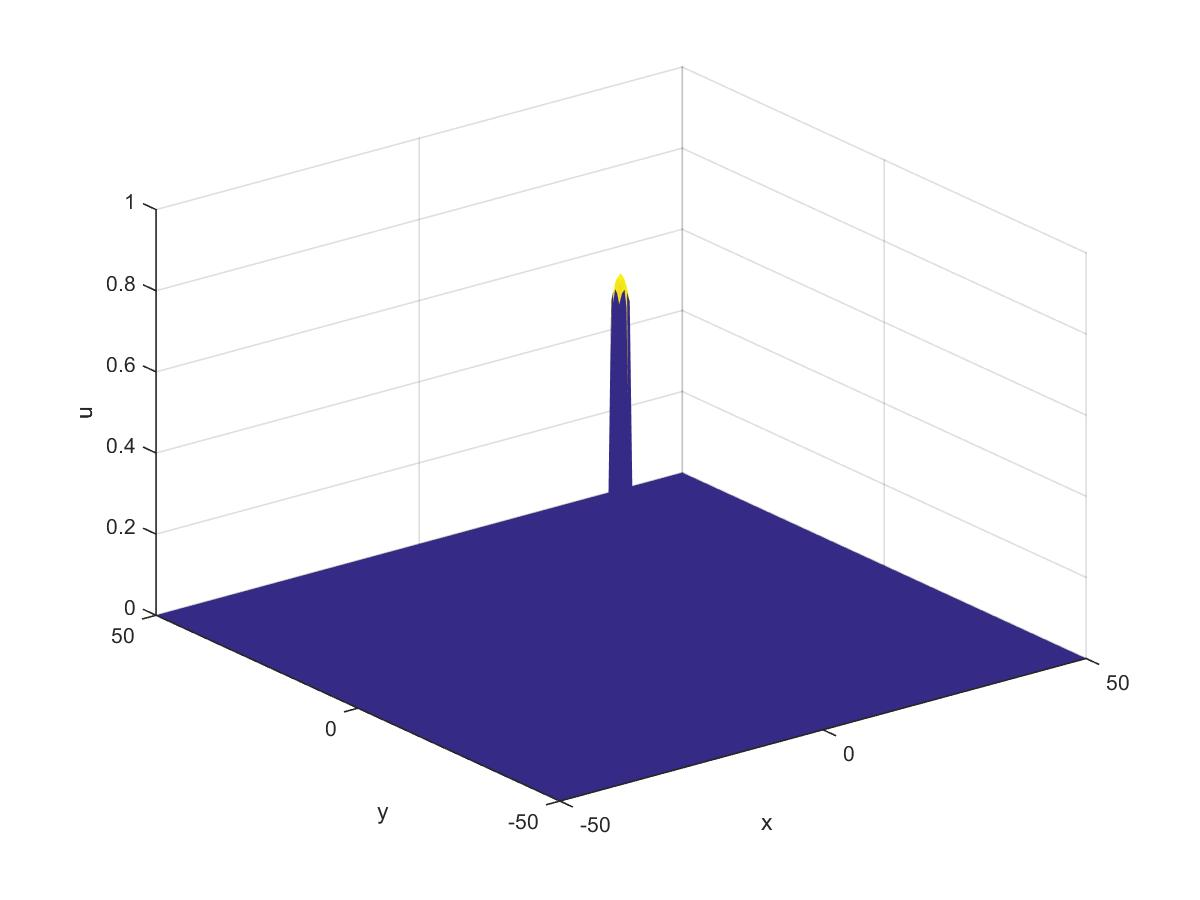
\includegraphics[width=0.3\linewidth]{Allee/333__1_}\hfill
    \includegraphics[width=0.3\linewidth]{Allee/333__2_}\hfill
	\includegraphics[width=0.3\linewidth]{Allee/333__3_}
    \caption{Diffusion 2D: t=0, t=500, t=5000}
\end{figure}
On se situe enfin dans le cas où $A=0.5$ et $u_0>A$. La vitesse de diffusion est toujours nulle et la densité initiale étant supérieure à la densité critique, la population va tendre vers l'état d'équilibre 1 sans diffuser. On aura donc une survie de la population dans une zone restreinte.

\subsubsection{Constante de diffusion d=0.05}
On diminue maintenant la constante de diffusion à 0.05 (ce qui consiste donc à diminuer l'impact de la diffusion):

\paragraph{Cas 2.1 : $d=0.05, A=0.25 (k=64), u_0=0.1$}
\noindent
\begin{figure}[H]
	\centering
	\includegraphics[width=0.40\linewidth]{Allee/F2211}\hfill
	\includegraphics[width=0.55\linewidth]{Allee/F4211}
    \caption{Diffusion 1D}
\end{figure}
\noindent
\begin{figure}[H]
	\centering
	\includegraphics[width=0.3\linewidth]{Allee/211__1_}\hfill
    \includegraphics[width=0.3\linewidth]{Allee/211__2_}\hfill
	\includegraphics[width=0.3\linewidth]{Allee/211__3_}
    \caption{Diffusion 2D: t=0, t=500, t=5000}
\end{figure}
On se situe dans le cas où $A<0.5$ et $u_0<A$. La population évolue sensiblement de la même manière que dans le cas 1.1. En effet, bien que la diffusion évolue, c'est ici l'effet Allee qui est responsable de l'extinction de la population, indépendemment de la diffusion.

\paragraph{Cas 2.2 : $d=0.05, A=0.25 (k=64), u_0=0.5$}
\noindent
\begin{figure}[H]
	\centering
	\includegraphics[width=0.40\linewidth]{Allee/F2212}\hfill
	\includegraphics[width=0.55\linewidth]{Allee/F4212}
    \caption{Diffusion 1D}
\end{figure}
\noindent
\begin{figure}[H]
	\centering
	\includegraphics[width=0.3\linewidth]{Allee/212__1_}\hfill
    \includegraphics[width=0.3\linewidth]{Allee/212__2_}\hfill
	\includegraphics[width=0.3\linewidth]{Allee/212__3_}
    \caption{Diffusion 2D: t=0, t=500, t=5000}
\end{figure}
On peut comparer ce cas au cas 1.2. On se situe en effet également à $A>0.5$ et $u_0>A$: La population va s'étendre et l'équilibre 1 va peu à peu envahir tout l'espace. Cependant, étant donné que la constante diffusion a diminué, cet envahissement sera beaucoup plus long à avoir lieu. Ceci explique que pour le même intervalle de temps, une surface plus petite soit occupée par notre population.

\paragraph{Cas 2.3 : $d=0.05, A=0.75 (k=7.1), u_0=0.5$}
\noindent
\begin{figure}[H]
	\centering
	\includegraphics[width=0.40\linewidth]{Allee/F2222}\hfill
	\includegraphics[width=0.55\linewidth]{Allee/F4222}
    \caption{Diffusion 1D}
\end{figure}
\noindent
\begin{figure}[H]
	\centering
	\includegraphics[width=0.3\linewidth]{Allee/222__1_}\hfill
    \includegraphics[width=0.3\linewidth]{Allee/222__2_}\hfill
	\includegraphics[width=0.3\linewidth]{Allee/222__3_}
    \caption{Diffusion 2D: t=0, t=500, t=5000}
\end{figure}
On se situe dans le cas où $A>0.5$ et $u_0<A$. Comme dans le cas 2.1, étant donné que nous sommes en présence d'un effet Allee fort, la valeur de la constante de diffusion a peu d'influence sur l'évolution de la population qui décroit rapidement jusqu'à l'extinction (comme dans le cas 1.3 avec les mêmes paramètres).

\paragraph{Cas 2.4 : $d=0.05, A=0.75 (k=7.1), u_0=0.9$}
\noindent
\begin{figure}[H]
	\centering
	\includegraphics[width=0.40\linewidth]{Allee/F2223}\hfill
	\includegraphics[width=0.55\linewidth]{Allee/F4223}
    \caption{Diffusion 1D}
\end{figure}
\noindent
\begin{figure}[H]
	\centering
	\includegraphics[width=0.3\linewidth]{Allee/223__1_}\hfill
    \includegraphics[width=0.3\linewidth]{Allee/223__2_}\hfill
	\includegraphics[width=0.3\linewidth]{Allee/223__3_}
    \caption{Diffusion 2D: t=0, t=500, t=5000}
\end{figure}
On se situe enfin dans le cas où $A>0.5$ et $u_0>A$. Comme dans le cas 1.4, la population va dans un premier temps augmenter pour atteindre l'équilibre 1. On devrait là aussi voir apparaitre une extinction de la population au bout d'un certain temps due à une vitesse de diffusion négative. Toutefois le taux de diffusion est trop faible pour que 0 puisse envahir 1 et on se retrouve dans un cas similaire au 1.6.

\subsection{Système de Lotka-Volterra}

Dans cette simulation, les paramètres sont choisis de façon à vérifier les hypothèses énoncées lors de l'analyse mathématique, à savoir : $\gamma_1 < \frac{K_1}{K_2}$ et $\gamma_2 > \frac{K_2}{K_1}$. On supposera de plus que $\alpha_1 = \alpha_2 = 0.6$ et que $K_1 = K_2 = 0.2$. On choisit donc $\gamma_1 = 0.5$ et $\gamma_2 = 1.5$.\\
Les constantes de diffusion sont $d_1 = 0.5$ (pour les Hommes Modernes) et $d_2 = 0.05$ (pour Néandertal).\\
On prend des densités de population initiales $u(0,0) = 0.03$ et $v(0,0) = K = 0.2$.

\begin{figure}[H]
\centering
\includegraphics[width=0.45\linewidth]{Comp/neand.png}
\includegraphics[width=0.45\linewidth]{Comp/homo.png}
\caption{Evolution des fronts d'onde au cours du temps}
\end{figure}

\begin{figure}[H]
\centering
\includegraphics[scale=0.3]{Comp/CompDiff2.png}
\caption{Diffusion 1D}
\end{figure}

La population d'Homo Sapiens croît très rapidement au cours du temps jusqu'à atteindre la capacité de soutien $K$, et grâce au phénomène de diffusion colonise également l'espace, ici représenté par une droite. La constante de diffusion choisie très faible pour Néandertal est responsable de la diminution rapide de la population.

\section{Interprétation biologique}

Les processus ayant mené à l'extinction de Néandertal ne sont pas encore parfaitement compris. Les données biologiques disponibles sont encore insuffisantes pour construire un modèle mathématique parfaitement pertinent.
De plus, les interactions de Néandertal avec Homo Sapiens sont complexes et pas encore bien connues. On sait que les deux espèces se sont croisées, hybridées, et que Néandertal a transmis à l'Homme Moderne une partie de son génôme.\\
Si le modèle de compétition choisi dans ce projet semble le plus pertinent, il ne rend pas compte de toute la complexité du monde vivant à cette époque, et des pressions de l'environnement qui ont influencé l'évolution de toutes les populations d'Homme.
\section{Bibliographie}
\begin{itemize}
    \item MURRAY J.D. Mathematical Biology, II : Spatial Models and Biomedical Applications. Springer.
    \item CURRAT M. EXCOFFIER L. (2004) Modern Humans Did Not Admix with Neanderthals during Their Range Expansion into Europe. PLoS Biol 2(12): e421. Disponible sur : \url{http://www.ncbi.nlm.nih.gov/pmc/articles/PMC532389/}
	\item V FABRE. Réponse démographique des Néandertaliens face aux pressions environnementales du stade isotopique3 : approche par modélisation écologique.[en ligne] Thèse Anthropologie Biologique. Aix-Marseille : Université d'Aix Marseille, 2011, 395p. Disponible sur : \url{ https://www.researchgate.net/publication/299411516_Reponse_demographique_des_Neandertaliens_face_aux_pressions_environnementales_du_stade_isotopique_3_approche_par_modelisation_ecologique}
	\item STEELE J. (2009). Human Dispersals: Mathematical Models and the Archaeological Record. Human Biology: Vol. 81: Iss. 2-3, Article 2. Disponible sur: \url{http://digitalcommons.wayne.edu/humbiol/vol81/iss2/2}
    \item UNIVERSITY OF CAMBRIDGE (2011) Teaching Reaction diffusion equations Michaelmas [en ligne]. Disponible sur : \url{https://homepage.univie.ac.at/marie-therese.wolfram/teaching.html} (consulté le 26.05.2016)
    \item A.KANDLER R.UNGER. Population Dispersal Via Diffusion-reaction Equations [en ligne].Techn. Univ., Fak. für Mathematik, 2010, 62p. Disponible sur \url{https://www-user.tu-chemnitz.de/~uro/publications/Kandler-Unger--Population_dispersal_via_diffusion-reaction_equations.pdf}
\end{itemize}

\section{Annexe}
\subsection{Démonstration Equation ~\eqref{Eq2}}

\[
\left\{
\begin{array}{r c l}
u(t,x)&=&U(z)\\
\frac{\partial u}{\partial t}&=&f(u(t,x))+d\Delta u(t,x)
\end{array}
\right.
\]

{\setlength{\baselineskip}{1.8\baselineskip}
\large{
\begin{itemize}[label=$\bullet$]
	\item $\frac{\partial u}{\partial t}(t,x)=\frac{dU}{dz}(z(t,x))\times\frac{dz}{dt}=U'(z)\times \frac{dz}{dt}=-c U'(z)$
    \item $\frac{\partial u}{\partial x}(t,x)=\frac{dU}{dz}(z(t,x))\times\frac{dz}{dx}=U'(z)\times \frac{dz}{dx}=U'(z)$
  	\item $\frac{\partial^2 u}{\partial x^2}(t,x)=\frac{d\dot U}{dz}(z(t,x))\times\frac{dz}{dx}=U"(z)$
\end{itemize}
}
\par}
Donc : $\eqref{Eq1}\Leftrightarrow -c U'(z)=d U"(z)+f(U(z))$

\end{document}